% Full working manuscript with the repository-audited Methodology and Experimental Design.
% The front matter and all other sections follow spectra.tex.
% This file is self-contained: it does not input the separate revised section fragment.
% Authors should resolve AUTHOR CHECK notes and revise the prose before submission.


%% 
%% Copyright 2007-2020 Elsevier Ltd
%% 
%% This file is part of the 'Elsarticle Bundle'.
%% ---------------------------------------------
%%


%% It may be distributed under the conditions of the LaTeX Project Public
%% License, either version 1.2 of this license or (at your option) any
%% later version.  The latest version of this license is in
%%    http://www.latex-project.org/lppl.txt
%% and version 1.2 or later is part of all distributions of LaTeX
%% version 1999/12/01 or later.
%% 
%% The list of all files belonging to the 'Elsarticle Bundle' is
%% given in the file `manifest.txt'.
%% 

%% Template article for Elsevier's document class `elsarticle'
%% with numbered style bibliographic references
%% SP 2008/03/01
%%
%% 
%%
%% $Id: elsarticle-template-num.tex 190 2020-11-23 11:12:32Z rishi $
%%
%%
\PassOptionsToPackage{dvipsnames}{xcolor}
% \documentclass[authoryear,preprint,12pt]{elsarticle}
% \documentclass[numbers,webpdf]{ima-authoring-template}%
% \documentclass[a4paper,fleqn]{cas-sc}

%% Use the option review to obtain double line spacing
% \documentclass[preprint,12pt]{elsarticle}

%% Use the options 1p,twocolumn; 3p; 3p,twocolumn; 5p; or 5p,twocolumn
%% for a journal layout:
%% \documentclass[final,1p,times]{elsarticle}
% \documentclass[authoryear,final,1p,times,twocolumn]{elsarticle}
% \documentclass[final,3p,times]{elsarticle}
% \documentclass[authoryear,final,3p,times,twocolumn]{elsarticle}
% \documentclass[final,5p,times]{elsarticle}
\documentclass[authoryear,final,5p,times,twocolumn]{elsarticle}

%% For including figures, graphicx.sty has been loaded in
%% elsarticle.cls. If you prefer to use the old commands
%% please give \usepackage{epsfig}

% --- Core color support ---
\usepackage{xcolor}
\usepackage{colortbl}

% \usepackage[style=authoryear, maxcitenames=1]{biblatex}
% \usepackage[authoryear]{natbib}

% --- Math ---
\usepackage{amsmath,amssymb,amsfonts,mathtools}
\usepackage{amsthm}

% --- Graphics & Tables ---
\usepackage{graphicx}
\usepackage{booktabs}
\usepackage{multirow}
\usepackage{makecell}
\usepackage{array}
\usepackage{tabularx}
\usepackage{arydshln}
\usepackage{adjustbox}
\usepackage{textcomp}
\usepackage{enumitem}

% --- Algorithms ---
\usepackage[linesnumbered,ruled,vlined]{algorithm2e}
\SetKwInput{KwInit}{Init}

% --- Floats ---
\usepackage{float}
\usepackage{placeins}
\usepackage{stfloats}

% --- Subfigures (elsarticle-safe) ---
\usepackage{subfig}   % NOT subcaption

% --- Boxes ---
\usepackage[most]{tcolorbox}

\usepackage{tikz}
\usetikzlibrary{
    arrows.meta,
    positioning,
    fit,
    calc,
    backgrounds,
    shapes.geometric
}

% --- Listings ---
\usepackage{listings}

% --- URLs / refs ---
\usepackage{xurl}
\usepackage{url}

% --- Hyperref LAST ---
\usepackage[colorlinks=true,
    linkcolor=MidnightBlue,
    citecolor=ForestGreen,
    urlcolor=BrickRed
]{hyperref}

\usepackage{pifont}
\newcommand{\cmark}{\textcolor{green!60!black}{\ding{51}}}
\newcommand{\xmark}{\textcolor{red}{\ding{55}}}
\newcommand{\method}{\textsc{SPECTRA-Siam}}
\newcommand{\concat}{\mathbin\Vert}
\newcommand{\relu}[1]{\left[#1\right]_{+}}
\newcommand{\todoauthor}[1]{\textcolor{red}{[AUTHOR CHECK: #1]}}
\newcommand{\degscore}[1]{%
  \cellcolor{red!10}#1\textsuperscript{\ensuremath{\dagger}}}
% Green marks content added to the original manuscript in this working copy.
\newcommand{\added}[1]{{\color{green!50!black}#1}}
% Keep the working manuscript compilable when draft figure files have not yet
% been uploaded to Overleaf.  Once a file is available, the real figure is used.
\newcommand{\safeincludegraphics}[2][]{%
  \IfFileExists{#2}{%
    \includegraphics[#1]{#2}%
  }{%
    \fbox{\parbox[c][3cm][c]{0.90\linewidth}{%
      \centering Missing draft figure:\\[-1mm]
      \texttt{\detokenize{#2}}%
    }}%
  }%
}

% --- Theorems ---
\newtheorem{theorem}{Theorem}
\newtheorem{assumption}{Assumption}
\newtheorem*{proofsketch}{Proof Sketch}
\theoremstyle{plain}

% --- Custom colors ---
\definecolor{titlegray}{HTML}{555555}
\definecolor{framegray}{gray}{0.6}
\definecolor{lightgray}{gray}{0.97}

% --- Prompt box ---
\newtcolorbox{promptbox}[1][]{
    enhanced,
    colback=lightgray,
    colframe=framegray,
    coltitle=white,
    colbacktitle=titlegray,
    fonttitle=\bfseries\itshape\normalsize,
    title=#1,
    attach boxed title to top left={xshift=0.6cm,yshift=-3mm},
    boxed title style={
        boxrule=0.8pt,
        colframe=titlegray,
        top=3pt,
        bottom=3pt,
        left=8pt,
        right=8pt,
        rounded corners=south,
    },
    width=0.90\columnwidth,
    before skip=6pt,
    after skip=12pt,
    boxrule=0.8pt,
    sharp corners=south,
    rounded corners,
    top=8pt,
    bottom=6pt,
    left=8pt,
    right=8pt,
    fontupper=\normalsize,
    coltext=black,
}

% --- Diff listings ---
\lstdefinelanguage{diff}{
  morecomment=[f][\color{gray}]{@@},
  morecomment=[f][\color{gray}]{---},
  morecomment=[f][\color{gray}]{+++},
  morecomment=[f][\color{red}]{-},
  morecomment=[f][\color{green!60!black}]{+},
}
\lstdefinestyle{diff}{
  language=diff,
  basicstyle=\ttfamily\footnotesize,
  columns=fullflexible,
  keepspaces=true,
  showstringspaces=false,
  breaklines=true
}
\definecolor{deepblue}{RGB}{0, 0, 139} 

\newtcolorbox{boxnote}{
  colback=white,
  boxrule=0.4pt,
  borderline west={2pt}{0pt}{black!60},
}

\renewcommand{\sectionautorefname}{Section}
\renewcommand{\subsectionautorefname}{Section}
\renewcommand{\subsubsectionautorefname}{Section}
\renewcommand{\algorithmautorefname}{Algorithm}
\renewcommand{\appendixautorefname}{Appendix}

\journal{Applied Soft Computing}

\begin{document}

\begin{frontmatter}

%% Title, authors and addresses

%% use the tnoteref command within \title for footnotes;
%% use the tnotetext command for theassociated footnote;
%% use the fnref command within \author or \address for footnotes;
%% use the fntext command for theassociated footnote;
%% use the corref command within \author for corresponding author footnotes;
%% use the cortext command for theassociated footnote;
%% use the ead command for the email address,
%% and the form \ead[url] for the home page:
%% \title{Title\tnoteref{label1}}
%% \tnotetext[label1]{}
%% \author{Name\corref{cor1}\fnref{label2}}
%% \ead{email address}
%% \ead[url]{home page}
%% \fntext[label2]{}
%% \cortext[cor1]{}
%% \affiliation{organization={},
%%             addressline={},
%%             city={},
%%             postcode={},
%%             state={},
%%             country={}}
%% \fntext[label3]{}

\title{Toward a Spectral Representation of Codes by Latent Graph Learning for Generalizable Semantic Code Clone Detection}

%% use optional labels to link authors explicitly to addresses:
%% \author[label1,label2]{}
%% \affiliation[label1]{organization={},
%%             addressline={},
%%             city={},
%%             postcode={},
%%             state={},
%%             country={}}
%%
%% \affiliation[label2]{organization={},
%%             addressline={},
%%             city={},
%%             postcode={},
%%             state={},
%%             country={}}

\author[mce]{Mohsen Hesamolhokama}
\ead{hokama@ce.sharif.edu}

\author[math]{Ali Sadeghi}
\ead{amirahmad.shafiee@sharif.edu}

\author[math]{Kousha Moeini}
\ead{amirahmad.shafiee@sharif.edu}

\author[math]{Behnam Rohani}
\ead{behnam.rohani058@sharif.edu}

\author[mce]{Mohammadamin Fazli}
\ead{fazli@sharif.edu}

\author[mce]{Jafar Habibi}
\ead{jhabibi@sharif.edu}

\address[mce]{Department of Computer Engineering, Sharif University of Technology, Tehran, Iran}
\address[math]{Department of Mathematical Sciences, Sharif University of Technology, Tehran, Iran}

% \cortext[cor1]{Corresponding author.}
% \fntext[fn1]{Authors Mohsen Hesamolhokama and Behnam Rohani contributed equally to this work.}

\begin{abstract}

\end{abstract}

% Use if graphical abstract is present
% \begin{graphicalabstract}
% \includegraphics{figs/grabs.pdf}
% \end{graphicalabstract}

\begin{keyword}
%% keywords here, in the form: keyword \sep keyword
%% PACS codes here, in the form: \PACS code \sep code
%% MSC codes here, in the form: \MSC code \sep code
%% or \MSC[2008] code \sep code (2000 is the default)
Code Representation \sep Graph Representation \sep Graph Spectral Analysis  \sep CCD \sep Code Similarity
\end{keyword}

\end{frontmatter}


\section{Introduction}
\label{sec:introduction}
% --- Paragraph 1: from source code to its representation to code clones ---
Nearly every automated task in software engineering begins with the same
artefact, the source code, and how useful that code is depends on how it is
represented \cite{allamanis2018survey}. A good representation makes it
possible to reason about what a program does, not only about how it is
written. This matters most when many tasks compare two pieces of code and
ask how similar they are. Code search retrieves functions that match a query
\cite{gu2018deepcs}. Plagiarism detection looks for reused fragments
across submissions \cite{schleimer2003winnowing}. Vulnerability analysis
looks for code that behaves like a known flawed pattern
\cite{zhou2019devign}. One of the most studied of these tasks is code
clone detection, which finds code fragments that are copies or that share
the same functionality. Clones are common in real systems, and they raise
maintenance cost because a change in one fragment often has to be repeated
in the others \cite{juergens2009clones,roy2007survey}. The quality of a
clone detector therefore depends, in the first place, on how well the
underlying representation captures the meaning of the code.

% --- Paragraph 2: methods for representing code; contrastive learning ---
How, then, should code be represented? Many answers have been proposed.
Early methods treat code as text or as a stream of tokens
\cite{schleimer2003winnowing}.
Because code also has structure, later methods use the abstract syntax
tree (AST) and encode it with tree-based neural networks
\cite{mou2016tbcnn}. Other methods learn distributed embeddings from code,
following the idea of word embeddings in natural language
\cite{mikolov2013word2vec,alon2019code2vec}. The Transformer architecture
\cite{vaswani2017attention} and pre-trained models such as BERT
\cite{devlin2019bert} were then adapted to code, which led to models like
CodeBERT \cite{feng2020codebert}, GraphCodeBERT
\cite{guo2021graphcodebert}, CodeT5 \cite{wang2021codet5}, and UniXcoder
\cite{guo2022unixcoder}. A key requirement of these representations is that
similar code should map to similar vectors. To enforce this, recent work
applies contrastive learning, which pulls equivalent code closer and
pushes different code apart \cite{chen2020simclr}. This idea has been used
for code through semantic-preserving transformations
\cite{jain2021contracode,bui2021corder} and through self-supervised
objectives over the AST \cite{bui2021infercode}. In short, similarity is
treated as a core property that the representation must encode.

% --- Paragraph 3: semantic clone detection and representation learning ---
Nowhere is this need for similarity sharper than in code clone detection,
the task we study. Clones are usually described in four types
\cite{roy2007survey}. The first three types cover identical or
syntactically similar code. The fourth type, the semantic clone, is code
that has the same functionality but a different syntax, and it is the
hardest to detect \cite{alomari2020semanticclonebench}. Representation
learning is now the main tool for this problem. Learned representations of
code have been used to detect clones with deep features
\cite{white2016deep,wei2017cdlh}, with AST-based encoders
\cite{zhang2019astnn}, with control-flow and data-flow features
\cite{zhao2018deepsim}, with token-level models
\cite{li2017cclearner}, and with graph neural networks over augmented
syntax trees \cite{wang2020faast,wu2020scdetector}. These methods are
evaluated on large benchmarks such as BigCloneBench
\cite{svajlenko2014bigclonebench}. The general lesson is simple. A
representation that can tell whether two fragments mean the same thing,
even when they look different, is a strong representation in general, and
it is exactly what semantic clone detection needs. Improving the
representation therefore improves clone detection directly.

% --- Paragraph 4: limits of current representations ---
Despite this progress, the representations we rely on today still fall short
in important ways. Pre-trained models such as CodeBERT have a fixed and
short input window, so they cannot read long functions, and self-attention grows quadratically with
the length of the input \cite{feng2020codebert,vaswani2017attention}. Work
on long inputs in natural language, such as Longformer
\cite{beltagy2020longformer} and BigBird \cite{zaheer2020bigbird}, shows
that this is a real constraint, and the problem is worse for code because
functions are often long. A second limit is that large language models
treat code as if it were ordinary text. Code is not only text. It has
explicit structure such as control flow and data dependence
\cite{hindle2012naturalness,allamanis2018survey}, and models that ignore
this structure do not capture program meaning well
\cite{chen2021codex,dou2023llmsurvey}. A third limit is generalization.
Deep models for clone detection tend to overfit their training data, and
their accuracy drops when they are tested on code from a different source
\cite{sonnekalb2022generalizability}. To use such a model on a new project,
one usually has to train it and then test it, which is costly. These
problems suggest a representation based on the graph of the code, which
keeps its structure, but comparing graphs directly is hard in its own way.
Exact graph and subgraph matching, such as graph edit distance, is
expensive to compute and returns only a distance, with no representation
that one can study further \cite{komondoor2001slicing}. Graph neural
networks avoid exact matching, but they again need training, add
computational cost, and can overfit because the models are complex
\cite{kipf2017gcn,xu2019gin}. \added{A graph spectrum provides an alternative
invariant summary: it can be computed by standard linear algebra, compared
without solving node correspondence, and approximated by retaining a bounded
number of eigenvalues \cite{chung1997spectral,defferrard2016cnngraph}. A raw
spectrum is not a complete graph invariant and its usefulness still depends on
the graph from which it is computed. This observation motivates our central
design choice: learning a task-relevant graph before constructing its spectral
descriptor.}

% --- Paragraph 5: our spectral approach ---
\added{Building on this observation, we propose \method{}, an end-to-end
Siamese model that learns the graph underlying a spectral source-code
representation. The observed AST and projected data-dependence relations are
normalized across languages and compressed into 32 latent nodes. The model then
infers a soft weighted adjacency and describes its normalized Laplacian through
eigenvalue density, heat traces, and differentiable Chebyshev spectral energies.
The density, heat-trace, and Chebyshev-energy blocks are normalized and compared
separately by a symmetric classifier. Pooled latent-node states, individual
embeddings, and raw lexical features do not bypass this spectral comparison.
The latent graph has fixed size, making descriptors comparable
across fragments, while its topology is optimized using semantic clone
supervision instead of being fixed as an AST, CFG, DDG, or CPG. Thus,
\method{} does require task-specific training; its ability to generalize beyond
the training distribution is evaluated explicitly through cross-dataset and
cross-language transfer experiments. The central question is whether learning
the graph on which the spectrum is defined yields a more discriminative and
transferable representation than spectra or neural encoders of predefined
program graphs.}

% %from source code to its representation to code clones
% Source code is the central artifact of software, and a large part of
% software engineering automation depends on how that code is represented
% \cite{allamanis2018survey}. A good representation makes it possible to
% reason about what a program does, not only about how it is written. This
% matters because many tasks compare two pieces of code and ask how similar
% they are. Code search retrieves functions that match a query
% \cite{gu2018deepcs}. Plagiarism detection looks for reused fragments
% across submissions \cite{schleimer2003winnowing}. Vulnerability analysis
% looks for code that behaves like a known flawed pattern
% \cite{zhou2019devign}. One of the most studied of these tasks is code
% clone detection, which finds code fragments that are copies or that share
% the same functionality. Clones are common in real systems, and they raise
% maintenance cost because a change in one fragment often has to be repeated
% in the others \cite{juergens2009clones,roy2007survey}. The quality of a
% clone detector therefore depends, in the first place, on how well the
% underlying representation captures the meaning of the code.

% %methods for representing code; contrastive learning
% Many ways to represent source code have been proposed. Early methods treat
% code as text or as a stream of tokens \cite{schleimer2003winnowing}.
% Because code also has structure, later methods use the abstract syntax
% tree (AST) and encode it with tree-based neural networks
% \cite{mou2016tbcnn}. Other methods learn distributed embeddings from code,
% following the idea of word embeddings in natural language
% \cite{mikolov2013word2vec,alon2019code2vec}. The Transformer architecture
% \cite{vaswani2017attention} and pre-trained models such as BERT
% \cite{devlin2019bert} were then adapted to code, which led to models like
% CodeBERT \cite{feng2020codebert}, GraphCodeBERT
% \cite{guo2021graphcodebert}, CodeT5 \cite{wang2021codet5}, and UniXcoder
% \cite{guo2022unixcoder}. A key requirement of these representations is that
% similar code should map to similar vectors. To enforce this, recent work
% applies contrastive learning, which pulls equivalent code closer and
% pushes different code apart \cite{chen2020simclr}. This idea has been used
% for code through semantic-preserving transformations
% \cite{jain2021contracode,bui2021corder} and through self-supervised
% objectives over the AST \cite{bui2021infercode}. In short, similarity is
% treated as a core property that the representation must encode.

% % semantic clone detection and representation learning
% Code clone detection is usually described in four types
% \cite{roy2007survey}. The first three types cover identical or
% syntactically similar code. The fourth type, the semantic clone, is code
% that has the same functionality but a different syntax, and it is the
% hardest to detect \cite{alomari2020semanticclonebench}. Representation
% learning is now the main tool for this problem. Learned representations of
% code have been used to detect clones with deep features
% \cite{white2016deep,wei2017cdlh}, with AST-based encoders
% \cite{zhang2019astnn}, with control-flow and data-flow features
% \cite{zhao2018deepsim}, with token-level models
% \cite{li2017cclearner}, and with graph neural networks over augmented
% syntax trees \cite{wang2020faast,wu2020scdetector}. These methods are
% evaluated on large benchmarks such as BigCloneBench
% \cite{svajlenko2014bigclonebench}. The general lesson is simple. A
% representation that can tell whether two fragments mean the same thing,
% even when they look different, is a strong representation in general, and
% it is exactly what semantic clone detection needs. Improving the
% representation therefore improves clone detection directly.


% % Why spectral and not just graph in general? Because:
% % 1. Distance over graph is costly to compute --> Graph-Edit Distance takes too much time for computation --> and they only give you the distance and no further insight as to representation
% % 2. GNN and graph neural networks need training and also computational cost and danger of overfitting since model complex
% % 3. Spectral can be computed like "the first k largest (absolute value)" first. There are linear-algebra algorithms for that --> approx possibility
% % 4. Spectral finger-print is more (a) natural, theoretical (b) can limited to only first k largest for more explained parts and save computational cost (c) it is underexplored and could be promising --> which we will show. (d) not fixed-length representation and SCALES with source code and graph length --> more promising to preserve info

% %limits of current representations
% Current learned representations still have important limits. Pre-trained
% models such as CodeBERT have a fixed and short input window, so they
% cannot read long functions, and self-attention grows quadratically with
% the length of the input \cite{feng2020codebert,vaswani2017attention}. Work
% on long inputs in natural language, such as Longformer
% \cite{beltagy2020longformer} and BigBird \cite{zaheer2020bigbird}, shows
% that this is a real constraint, and the problem is worse for code because
% functions are often long. A second limit is that large language models
% treat code as if it were ordinary text. Code is not only text. It has
% explicit structure such as control flow and data dependence
% \cite{hindle2012naturalness,allamanis2018survey}, and models that ignore
% this structure do not capture program meaning well
% \cite{chen2021codex,dou2023llmsurvey}. A third limit is generalization.
% Deep models for clone detection tend to overfit their training data, and
% their accuracy drops when they are tested on code from a different source
% \cite{sonnekalb2022generalizability}. To use such a model on a new project,
% one usually has to train it and then test it, which is costly. What is
% missing is a method that does not need this training, that has lower time
% cost, and that does not suffer from the problems above.

% % our spectral approach
% To address these limits, we propose a method based on spectral analysis of
% source code. We build a custom graph of each code fragment so that the
% graph reflects both the structure and the behaviour of the code. We then
% describe the fragment through the spectrum of this graph, that is, through
% the eigenvalues of its associated matrix. The spectrum gives a fixed-size
% description of the whole graph and does not change when the nodes are
% relabelled, which is useful for comparing graphs of different sizes
% \cite{narayanan2017graph2vec,xu2019gin}. This gives a representation that
% shows the similarities and the differences between fragments and that can
% be used directly for clone detection. Our method does not require model
% training, so it does not have the overfitting problem and does not need a
% separate train-and-test step for each dataset. It is also much faster than
% heavy graph neural network models \cite{hamilton2017graphsage}. The central
% question we study is which graph of the code yields the most informative
% spectrum. We judge a graph by how well its spectrum reflects the semantic
% meaning of the code, and we use this criterion to guide the design of our
% representation for code clone detection.


\definecolor{kwcolor}{RGB}{0,0,180}
\definecolor{cmtcolor}{RGB}{0,128,0}
\definecolor{strcolor}{RGB}{170,0,0}
\definecolor{bgcolor}{RGB}{248,248,248}
\lstdefinestyle{javastyle}{
  language=Java, basicstyle=\scriptsize\ttfamily,
  keywordstyle=\color{kwcolor}\bfseries, commentstyle=\color{cmtcolor}\itshape,
  stringstyle=\color{strcolor}, numberstyle=\tiny\color{gray},
  backgroundcolor=\color{bgcolor}, frame=single, framesep=2pt,
  showstringspaces=false, breaklines=true, columns=fullflexible, keepspaces=true,
  aboveskip=2pt, belowskip=2pt,
}

\subsection{A Motivating Example}
\label{sec:motivating_exp}

\begin{figure*}[t]
\centering
% ----------------------- row 1: the three code fragments -----------------
\begin{minipage}[t]{0.32\linewidth}
\begin{lstlisting}[style=javastyle,caption={A: sum with a for loop.},label={lst:for}]
int sumArray(int[] a) {
    int s = 0;
    for (int i=0; i<a.length; i++)
        s += a[i];
    return s;
}
\end{lstlisting}
\end{minipage}\hfill
\begin{minipage}[t]{0.32\linewidth}
\begin{lstlisting}[style=javastyle,caption={B: sum with a while loop.},label={lst:while}]
int aggregate(int[] v) {
    int acc = 0, k = 0;
    while (k < v.length) {
        int x = v[k];
        acc = acc + x;
        k = k + 1;
    }
    return acc;
}
\end{lstlisting}
\end{minipage}\hfill
\begin{minipage}[t]{0.32\linewidth}
\begin{lstlisting}[style=javastyle,caption={C: triangle area (unrelated).},label={lst:area}]
double area(double x,
            double y, double z) {
    double s = (x+y+z)/2;
    double p = s*(s-x);
    double q = p*(s-y);
    double r = q*(s-z);
    return Math.sqrt(r);
}
\end{lstlisting}
\end{minipage}

\vspace{4pt}
% ------------- row 2: small graphs (left) + barcode (right) ----------------
\begin{minipage}[c]{0.70\linewidth}
\centering
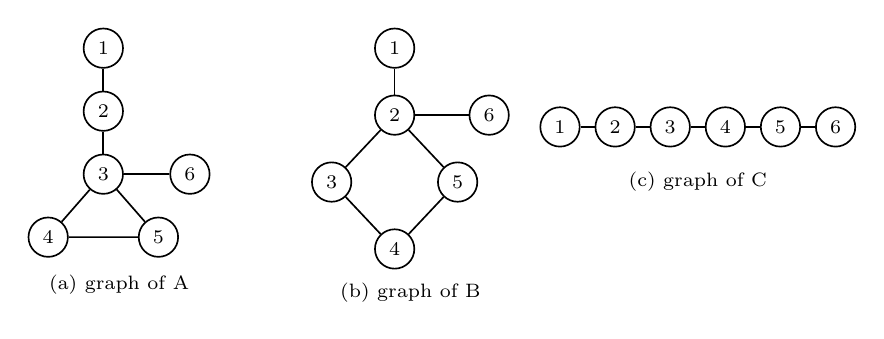
\begin{tikzpicture}[
   vtx/.style={circle,draw,semithick,fill=white,minimum size=5mm,inner sep=0pt,font=\scriptsize},
   every path/.style={semithick}]
  % A: 3-node loop
  \node[vtx](a1) at (0,0){1};   \node[vtx](a2) at (0,-0.8){2};
  \node[vtx](a3) at (0,-1.6){3}; \node[vtx](a6) at (1.1,-1.6){6};
  \node[vtx](a4) at (-0.7,-2.4){4}; \node[vtx](a5) at (0.7,-2.4){5};
  \draw (a1)--(a2)--(a3); \draw (a3)--(a4)--(a5)--(a3); \draw (a3)--(a6);
  \node[font=\scriptsize] at (0.2,-3.0){(a) graph of A};
  % B: 4-node loop (diamond)
  \begin{scope}[xshift=37mm]
    \node[vtx](b1) at (0,0){1};      \node[vtx](b2) at (0,-0.85){2};
    \node[vtx](b6) at (1.2,-0.85){6};
    \node[vtx](b3) at (-0.8,-1.7){3}; \node[vtx](b5) at (0.8,-1.7){5};
    \node[vtx](b4) at (0,-2.55){4};
    \draw (b1)--(b2); \draw (b2)--(b6); \draw (b2)--(b3)--(b4)--(b5)--(b2);
    \node[font=\scriptsize] at (0.2,-3.1){(b) graph of B};
  \end{scope}
  % C: horizontal chain (no loop)
  \begin{scope}[xshift=58mm, yshift=-1.0cm]
    \node[vtx](c1) at (0,0){1};   \node[vtx](c2) at (0.7,0){2};
    \node[vtx](c3) at (1.4,0){3}; \node[vtx](c4) at (2.1,0){4};
    \node[vtx](c5) at (2.8,0){5}; \node[vtx](c6) at (3.5,0){6};
    \draw (c1)--(c2)--(c3)--(c4)--(c5)--(c6);
    \node[font=\scriptsize] at (1.75,-0.7){(c) graph of C};
  \end{scope}
\end{tikzpicture}
\end{minipage}\hfill
\begin{minipage}[c]{0.27\linewidth}
\centering
% grayscale barcode: darkness = lambda / lambda_max, lambda_max = 5.236
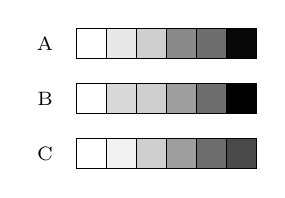
\begin{tikzpicture}[every path/.style={thin}]
  \def\cw{0.38}
  \node[font=\scriptsize] at (-0.4,0)    {A};
  \foreach \i/\p in {0/0,1/9,2/19,3/46,4/57,5/97}
     {\fill[black!\p] (\i*\cw,-0.19) rectangle ++(\cw,0.38);
      \draw (\i*\cw,-0.19) rectangle ++(\cw,0.38);}
  \node[font=\scriptsize] at (-0.4,-0.7) {B};
  \foreach \i/\p in {0/0,1/15,2/19,3/38,4/57,5/100}
     {\fill[black!\p] (\i*\cw,-0.89) rectangle ++(\cw,0.38);
      \draw (\i*\cw,-0.89) rectangle ++(\cw,0.38);}
  \node[font=\scriptsize] at (-0.4,-1.4) {C};
  \foreach \i/\p in {0/0,1/5,2/19,3/38,4/57,5/71}
     {\fill[black!\p] (\i*\cw,-1.59) rectangle ++(\cw,0.38);
      \draw (\i*\cw,-1.59) rectangle ++(\cw,0.38);}
\end{tikzpicture}\\[2pt]
{\scriptsize spectrum as a barcode\\(each cell $=\lambda_i$, darker $=$ larger)}
\end{minipage}

\caption{Three Java fragments, their graphs, and their spectra as a
grayscale barcode. A and B both sum an array and are clones, but A has a
three-node loop and B a four-node loop, so their graphs differ. Their
barcodes still look almost the same, while the unrelated function C, which
has no loop, is lighter in the last cell.}
\label{fig:motivating_exp}
\end{figure*}

Figure~\ref{fig:motivating_exp} shows two Java functions that both sum an
integer array, written with a different loop and different variable names,
together with an unrelated function C that computes a triangle area. As
text, A and B share no identifiers, so token- or line-based comparison
finds little in common between them
\cite{roy2007survey,alomari2020semanticclonebench}. Their graphs are also
not identical: A has a three-node loop and B a four-node loop. Yet if we
take the spectrum (the sorted Laplacian eigenvalues) as the signature of
each graph, A gives $\{0,\,0.485,\,1.000,\,2.425,\,3.000,\,5.089\}$ and B
gives $\{0,\,0.763,\,1.000,\,2.000,\,3.000,\,5.236\}$, which are close, as
the barcodes in the figure show. The unrelated function C gives
$\{0,\,0.268,\,1.000,\,2.000,\,3.000,\,3.732\}$, whose top eigenvalue is
much smaller, so its barcode is visibly lighter. Measuring similarity as the
Euclidean distance between sorted spectra gives $0.53$ for the clone pair
and $1.44$ and $1.58$ for the two non-clone pairs, so a simple threshold
separates them. Because the spectrum is invariant to node relabelling and
changes only a little under small edits to the graph, it matches
behaviourally equivalent code that looks different on the surface. This
motivates our approach and raises its central question: which graph of the
code yields the most informative spectrum for clone detection.

\subsection{Contributions}
\label{subsec:contributions}

The main contributions of this paper are as follows:

\begin{itemize}
    \item \textbf{End-to-End Spectral Representation through Latent Graph
    Learning}: We propose a learnable spectral code representation in which a
    fixed-size, weighted latent graph is induced from AST-derived structural
    information. Its normalized Laplacian representation is optimized under
    semantic clone supervision, eliminating the need to select an AST, CFG,
    DDG, or CPG as the final spectral graph.

    \item \textbf{Semantic Alignment of Latent Graph Spectra through Clone
    Supervision}: A Siamese architecture jointly exploits spectral and latent
    structural information to bring functionally equivalent programs closer
    while separating non-equivalent ones.

    \item \added{\textbf{Language-Normalized Multi-Scale Spectral Encoding}:
    We combine canonical AST-node categories, AST and projected-DDG relations,
    soft slot-based graph induction, eigenvalue-density and heat-trace summaries,
    and differentiable Chebyshev spectral energies.}

    \item \added{\textbf{Controlled Evaluation and Generalization}: We compare
    the learned graph with fixed spectral representations, observed-graph GNNs,
    non-graph, graph-based, hybrid, and independently implemented pretrained
    baselines on four prepared clone benchmarks. Latent-capacity and three-arm
    feature ablations isolate the main design choices. We additionally evaluate
    zero-shot cross-dataset transfer and source-to-target language transfer with
    the source-selected model and threshold kept fixed.}
\end{itemize}

% For Mohsen to write the first-version

% Proposing a new graph design for source codes that gives us a good spectral representation --> (a) better than AST, CFG, PDG, DDG, etc (traditional graph representations) judged over code clone benchmarks and how good we score. Also, (b) further analysis and backing of the good graph design made by us.

% Empirical study and Exploration of spectral representation over "different graphs of code" on "diverse set of datasets" in "both single-language and cross-language" compared with "Statistical Token based feature space" and "CodeBert Transformer-type embeddings" and "various other CCD approaches that are trained (not baseline but previous work)" using "different metrics" and "eigenvalue + eigenvector" through "other variable and experiments".

% Analytical and a thorough investigation of spectral representation space of source codes and insights and projection operators over that space. --> Eigenvectors and how they can be used for spectral representations in general.

\subsection{Paper Organization}
\label{subsec:outline}

The rest of this paper is organized as follows. \autoref{sec:related_work} reviews related work on code clone
detection, source code representation, and spectral analysis of graphs, and
\autoref{sec:motivating_exp} gives a motivating example. We then present our
graph design and spectral representation, followed by the experimental
setup and the results on single-language and cross-language benchmarks.
Finally, we analyse the spectral representation space and conclude with a
summary and directions for future work.


\section{Related Work}
\label{sec:related_work}

% Our work builds on three lines of research. The first is code clone
% detection. The second is source code representation. The third is
% spectral analysis of graphs. We first review how clone detection has
% moved from text and token matching to learning and graph based semantic
% methods (\autoref{subsec:ccd}). We then describe how source code is
% encoded into the structural and learned representations that detectors
% rely on (\autoref{subsec:representation}). After that we summarise the
% theory and the main applications of graph spectral analysis in other
% fields (\autoref{subsec:spectral}). This last part motivates our use
% of the graph spectrum as a signature of code structure that does not
% depend on node ordering. We close by positioning our contribution against
% this body of work (\autoref{subsec:gap}).

% ---------------------------------------------------------------------
\subsection{Code Clone Detection}
\label{subsec:ccd}

Code clone detection has been studied for more than two decades. Most
techniques are grouped by the program representation on which similarity
is measured. Roy and Cordy \cite{roy2007survey} classify clones into four
types. Type-1 clones are identical except for formatting and naming.
Type-2 and Type-3 clones are syntactically similar but contain small
changes. Type-4 clones implement the same functionality with different
syntax.

\textbf{Text and token based approaches.} The earliest scalable detectors
work on lexical information. \emph{CCFinder} \cite{kamiya2002ccfinder}
normalises token sequences and compares them across several languages.
Ducasse et al.\ \cite{ducasse1999language} detect duplicated code by
matching lines in a language independent way. \emph{CP-Miner}
\cite{li2006cpminer} mines copy-paste bugs in large systems.
\emph{NICAD} \cite{roy2008nicad} adds flexible pretty-printing to line
based comparison so that it can capture near-miss clones. To handle very
large code bases, several token based detectors add indexing and
filtering. \emph{SourcererCC} \cite{sajnani2016sourcerercc} uses an
inverted index. \emph{CCAligner} \cite{wang2018ccaligner} uses
overlapping code windows. \emph{Oreo} \cite{saini2018oreo} uses metric
based filtering. More recently, \emph{StoneDetector}
\cite{heinze2025stonedetector} compares paths taken from dominator trees
of Java source and bytecode. These methods scale well. However, they
mostly ignore code structure, so they have trouble with Type-3 and
Type-4 clones.

\textbf{Tree and graph based approaches.} To capture structural
similarity, detectors began to use the abstract syntax tree (AST).
Baxter et al.\ \cite{baxter1998clone} match subtrees of the AST.
\emph{DECKARD} \cite{jiang2007deckard} describes subtrees with numerical
vectors and clusters them in Euclidean space. Some clones survive
statement reordering or interleaving, which lexical and tree methods miss.
This motivated graph based detectors. Komondoor and Horwitz
\cite{komondoor2001slicing} and Krinke \cite{krinke2001identifying} search
for isomorphic subgraphs of the program dependence graph (PDG). The PDG
uses control flow and data flow rather than surface syntax. Subgraph
isomorphism is expensive to compute, which has limited the scalability of
PDG based methods.

\textbf{Learning and deep learning based approaches.} A large body of
recent work learns similarity directly from data. White et al.\
\cite{white2016deep} were among the first to apply deep learning to clone
detection. They link lexical patterns with syntactic patterns. The
\emph{CDLH} framework \cite{wei2017cdlh} treats functional clone detection
as a supervised hashing problem over AST based LSTMs. \emph{ASTNN}
\cite{zhang2019astnn} splits an AST into statement subtrees and encodes
them with recurrent networks. Tree based convolution
\cite{yu2019neural} and recursive aggregation of ASTs
\cite{buch2019learning} are other structural encoders. Graph neural
networks (GNNs) reduce the semantic gap further. The flow augmented AST
(\emph{FA-AST}) of Wang et al.\ \cite{wang2020faast} adds control flow and
data flow edges to the AST and applies GNNs to measure pairwise
similarity. Graph based semantics learning \cite{yu2023graphsemantics}
combines CFG and PDG representations with attention based graph matching.
\emph{FSD-CLCD} \cite{zhang2024fsdclcd} addresses cross-language detection
through functional semantic distillation over AST derived graphs. Other
work targets efficiency. Transformer based detectors with code token
learners \cite{zhang2023efficient} reduce the cost of attention.
\emph{CCStokener} \cite{wang2023ccstokener} adds semantic information to
tokens. \emph{Code2Img} \cite{hu2023code2img} turns the AST adjacency
matrix into an image and processes it with convolutional networks. The
\emph{BigCloneBench} benchmark \cite{svajlenko2014bigclonebench} is the
standard dataset for evaluating these detectors at scale.

These detectors are accurate, but they have practical costs. GNN and
Transformer based methods need large labelled datasets. They also rely on
costly pairwise comparison and expensive training. In addition, the
learned similarity is often sensitive to node ordering and to graph size.
These limitations motivate representations of code structure that are
compact and do not need heavy training.

% ---------------------------------------------------------------------
\subsection{Source Code Representation}
\label{subsec:representation}

The performance of a clone detector depends heavily on how source code is
represented. The classical representations are explicit program
structures. The AST captures syntax. The control flow graph (CFG) and the
PDG capture execution and dependence relations. The code property graph
(CPG) of Yamaguchi et al.\ \cite{yamaguchi2014cpg} joins syntax, control
flow, and data flow in a single graph, and it has proven effective for
finding vulnerabilities. These graph representations keep rich semantic
information. They are also high dimensional and irregular, which makes
direct comparison difficult.

A second line of work learns continuous representations of code.
\emph{code2vec} \cite{alon2019code2vec} aggregates AST paths into a fixed
length embedding that predicts semantic properties of a snippet.
Pre-trained language models extend this idea to large corpora.
\emph{CodeBERT} \cite{feng2020codebert} learns joint representations of
programming language and natural language. \emph{GraphCodeBERT}
\cite{guo2021graphcodebert} adds data flow structure to the pre-training
objective and improves downstream tasks such as clone detection.
Structure aware neural encoders such as ASTNN \cite{zhang2019astnn} and
FA-AST \cite{wang2020faast} can also be seen as representation learners.
These embeddings are powerful. However, they are learned end to end, they
depend on their training distribution, and they are hard to interpret. In
contrast, our work derives a representation from the algebraic structure
of the code graph itself, so it does not require supervised pre-training.

% ---------------------------------------------------------------------
\subsection{Spectral Analysis of Graphs}
\label{subsec:spectral}

Spectral graph theory studies a graph through the eigenvalues and
eigenvectors of matrices associated with it. The two main matrices are the
adjacency matrix and the graph Laplacian
\cite{chung1997spectral,mohar1991laplacian}. The spectrum encodes global
properties of the graph. Fiedler \cite{fiedler1973algebraic} showed that
the second smallest Laplacian eigenvalue, known as the algebraic
connectivity, measures how well connected a graph is. This result is a
basis for much of modern spectral analysis. The set of eigenvalues does
not change when the vertices are relabelled. This makes the spectrum a
natural signature for comparing graphs of different sizes, which is the
property that AST and PDG comparison needs.

Spectral methods have been successful in many fields. In unsupervised
learning, normalized cuts \cite{shi2000normalized} and the spectral
clustering algorithms of Ng et al.\ \cite{ng2002spectral} and von Luxburg
\cite{vonluxburg2007tutorial} partition data using the leading Laplacian
eigenvectors. In manifold and dimensionality reduction, Laplacian
eigenmaps \cite{belkin2003laplacian} preserve local geometry through the
same eigenbasis. In computer vision and graphics, spectral correspondence
\cite{leordeanu2005spectral} solves matching problems using the principal
eigenvector of an affinity matrix. The heat kernel signature
\cite{sun2009hks} and spectral mesh processing
\cite{zhang2010spectralmesh} use the Laplace--Beltrami spectrum as a shape
descriptor that does not change under isometric deformation. In graph
mining, Weisfeiler--Lehman graph kernels \cite{shervashidze2011wl} compare
graphs through structural features that are refined step by step. Spectral
theory is also the basis of modern graph deep learning. Spectral networks
\cite{bruna2014spectral}, fast localized spectral filtering with Chebyshev
polynomials \cite{defferrard2016cnngraph}, and the graph convolutional
network \cite{kipf2017gcn} all define convolution through the graph
Laplacian spectrum. Later work generalised these ideas with attention
based models \cite{velickovic2018gat}.

The common lesson across these fields is that the graph spectrum gives a
compact description of structure that does not depend on node ordering.
Graph representations of source code are widely used. Even so, the
explicit use of spectral signatures of code graphs for clone detection
has received little attention.

% ---------------------------------------------------------------------
\subsection{Positioning of Our Work}
\label{subsec:gap}

We can summarise the trade-offs as follows. Token and tree based detectors
scale well, but they miss semantic clones. GNN and Transformer based
detectors capture semantics, but they need large labelled corpora and
expensive training, and they are sensitive to graph size and node
ordering. \added{Spectral graph analysis supplies a compact, permutation-invariant
description of global structure, but a spectrum computed from an unsuitable
program graph can discard task-relevant semantics. We therefore do not treat
spectral analysis as a training-free replacement for learning. Instead, we make
the latent graph itself learnable and use clone supervision to determine the
topology on which a multi-scale spectral descriptor is computed. Fixed-graph
spectral methods remain as explicit controls, allowing the experiments to
separate the contribution of spectral comparison from the contribution of
task-guided graph induction.}


\section{Methodology}
\label{sec:methodology}

\subsection{Motivation}
\label{sec:methodology_motivation}

\added{A conventional spectral pipeline fixes the program graph before the
clone-detection objective is known. Consequently, the extracted spectrum can
express only the relations encoded by that selected graph view. Our objective
is to preserve the ordering invariance and global structural summary offered by
spectral analysis while allowing clone supervision to determine the graph on
which the representation is computed.}

\method{} learns the graph on which a spectral code representation is computed.
For each source-code fragment, the model first maps parser-specific node types to
a shared structural vocabulary, encodes the available syntactic and data-dependence
relations, and compresses the variable-size input graph into a fixed number of
latent nodes. It then infers a weighted latent adjacency, represents the resulting
graph at several spectral scales, and fuses the spectral descriptor with pooled
latent-node states. Two fragments are processed by a shared encoder, and a pairwise
head estimates whether they implement the same functionality.

This design separates two roles that are conflated in a conventional graph-spectral
pipeline. The observed AST and DDG provide evidence about program structure, while
the graph used for the final spectral representation is induced for the clone
detection objective rather than selected a priori.

\begin{figure*}[t]
    \centering
    \safeincludegraphics[width=0.95\textwidth]{figures/main_fig.png}
    \caption{\method{} architecture. A shared encoder maps each fragment to a
    common representation by normalizing its observed program graph, inducing
    a weighted latent graph, extracting a multi-scale spectral descriptor, and
    fusing spectral and latent features. The pairwise head estimates semantic
    clone probability.}
    \label{fig:spectra_overview}
\end{figure*}

\subsection{Problem Formulation}
\label{sec:problem_formulation}

Let $\mathcal{L}$ be the set of programming languages and let
$\mathcal{C}_{\ell}$ contain the code fragments written in language
$\ell\in\mathcal{L}$. For a pair $(c_i,c_j)$, the label
$y_{ij}\in\{0,1\}$ indicates functional equivalence:
\begin{equation}
y_{ij}=
\begin{cases}
1, & c_i\equiv_{\mathrm{func}}c_j,\\
0, & \text{otherwise}.
\end{cases}
\label{eq:clone_label}
\end{equation}
The task is therefore semantic clone detection rather than direct lexical or
syntactic matching.

A fixed spectral method applies a predetermined graph constructor
$\mathcal{G}_{b}$ and a spectral transform:
\begin{equation}
c\xrightarrow{\mathcal{G}_{b}}G_b(c)
\xrightarrow{\operatorname{Spec}}s_b(c),
\label{eq:fixed_spectrum}
\end{equation}
where $b$ denotes an observed program-graph view. In contrast, \method{} learns
\begin{equation}
G_{\Theta}(c)=\bigl(Z_{\Theta}(c),A_{\Theta}(c)\bigr),
\label{eq:learned_graph}
\end{equation}
where $Z_{\Theta}(c)\in\mathbb{R}^{m\times d}$ contains $m$ latent-node
states and $A_{\Theta}(c)\in[0,1]^{m\times m}$ is a weighted adjacency.
The shared encoder produces
\begin{equation}
\begin{aligned}
\phi_{\Theta}(c)
&=F_{\Theta}\!\left(
Z_{\Theta}(c),
\operatorname{Spec}_{\Theta}(G_{\Theta}(c))
\right),
\end{aligned}
\label{eq:code_embedding}
\end{equation}
and a pairwise head $f_{\psi}$ gives
\begin{equation}
\widehat{p}_{ij}=f_{\psi}\bigl(\phi_{\Theta}(c_i),
\phi_{\Theta}(c_j)\bigr).
\label{eq:pair_probability_general}
\end{equation}

\subsection{Input Graph Construction and Language Normalization}
\label{sec:input_representation}

\paragraph{Observed graph relations.}
The preprocessing pipeline exports AST, CFG, DDG, and CPG views. The main
\method{} configuration does not consume all four views. It uses the AST and a
DDG projected onto the AST node namespace. \added{A DDG edge is retained only
when both endpoint identifiers can be matched to AST nodes; retained DDG edges
are made bidirectional. AST edges are likewise symmetrized before batching. The
implementation also constructs a bidirectional sequential relation between
adjacent serialized AST nodes, but this relation is disabled in every reported
main \method{} run.} Thus, the principal relation set is
\begin{equation}
\mathcal{R}_{\mathrm{main}}=\{\mathrm{AST},\mathrm{DDG}\}.
\label{eq:main_relations}
\end{equation}
\added{The zero-shot cross-language experiment uses the same AST+DDG relation
set. A projected DDG edge is included only when both endpoints align with the
AST namespace; absent projected edges therefore remain empty rather than
silently changing the configured relation set. No VST representation is
present, and PDG is not included in the reported experiment artifacts.}

\paragraph{Canonical node categories.}
Parser-specific node names are mapped to a fixed set of 24 categories:
\begin{quote}\small
Control\_If, Control\_Loop, Control\_Switch, Control\_Return,
Control\_Break, Control\_Generic, Var\_Decl, Func\_Decl,
Class\_Decl, Param\_Decl, Assign\_Op, Binary\_Op, Unary\_Op,
Call\_Expr, Access\_Expr, Literal\_Num, Literal\_Str,
Literal\_Bool, Literal\_Null, Literal\_Generic, Structural\_Block,
Identifier\_Context, Type\_Meta, and Canonical\_Unknown.
\end{quote}
\added{The mapping covers aliases emitted by Joern, Python's AST parser, and the
language-specific fallbacks used by the data pipeline. Ambiguous parser labels
are mapped conservatively to a generic or unknown category rather than inferred
from the evaluation data.}

\paragraph{Bounded lexical sketch.}
Each node may additionally receive a small, vocabulary-free lexical sketch.
\added{Non-numeric labels are split at punctuation and camel-case boundaries,
literal values are normalized, and the first subtokens and character trigrams
are mapped deterministically into 4,096 hash buckets, with at most four hashed
features retained per node. Pure line-number labels are ignored. This sketch is distinct from the optional hashed source-token
residual: the latter hashes source-code tokens into 96 slots and is disabled in
the canonical configuration.}

For node $v$, let $\kappa(t_v)$ be its canonical category and let
$\ell_{v1},\ldots,\ell_{vr}$ be its hashed node-label features. The initial
state is
\begin{equation}
\begin{aligned}
h_v^{(0)}
&=\operatorname{LN}\!\left(
E_{\mathrm{can}}(\kappa(t_v))
+\gamma_{\mathrm{lex}}\frac{1}{r}
\sum_{q=1}^{r}E_{\mathrm{lex}}(\ell_{vq})
\right),\\
\gamma_{\mathrm{lex}}
&=\sigma(g_{\mathrm{lex}}).
\end{aligned}
\label{eq:node_initialization}
\end{equation}
\added{The lexical gate is learned and is initialized to approximately $0.20$.
Node-label features are dropped with probability $0.30$ during training. Graphs
are truncated to the first 256 serialized AST nodes, and a mask prevents padded
nodes from contributing to message passing or reconstruction.}

\subsection{Relation-Aware Structural Encoding}
\label{sec:relation_encoder}

Let $H^{(l)}\in\mathbb{R}^{n\times d}$ denote node states at layer $l$ and
let $A^{(r)}$ be the adjacency of relation $r$. A relation-aware layer computes
\begin{equation}
\begin{aligned}
H^{(l+1)}
&=\operatorname{LN}\!\left[
H^{(l)}+\operatorname{Dropout}\!\left(
\operatorname{GELU}(U^{(l)})
\right)\right],\\
U^{(l)}
&=H^{(l)}W_0^{(l)}+
\sum_{r\in\mathcal{R}}
\widetilde{A}^{(r)}H^{(l)}W_r^{(l)}.
\end{aligned}
\label{eq:relation_layer}
\end{equation}
where $\widetilde{A}^{(r)}$ is row-normalized. \added{The implementation uses a
degree floor of one in this normalization.}
The encoder uses two such layers, hidden dimension $d=256$, and dropout $0.10$.

\subsection{Latent Graph Induction}
\label{sec:latent_induction}

The encoded program graph has a fragment-dependent number of nodes. Iterative
slot attention maps it to $m$ fixed latent nodes. With normalized input keys
$k_v$, slot queries $q_j$, and mask $M_v$, the implementation first normalizes
assignments over slots,
\begin{equation}
P_{vj}=
\frac{\exp(q_j^{\top}k_v/\sqrt{d})}
{\sum_{u=1}^{m}\exp(q_u^{\top}k_v/\sqrt{d})},
\label{eq:slot_assignment}
\end{equation}
then normalizes each slot over input nodes before aggregating values. Slot states
are updated by a GRU followed by a residual MLP. \added{This second normalization
and the GRU--MLP update are part of the implemented slot-attention block.} The
canonical configuration uses $m=32$ slots and three iterations.

The assignment matrix reconstructs the input features as $\widehat{H}=PZ$. The
masked reconstruction objective is
\begin{equation}
\mathcal{L}_{\mathrm{rec}}=
\frac{1}{\sum_v M_v}
\sum_v M_v\frac{1}{d}\left\|h_v^{(0)}-\widehat{h}_v\right\|_2^2.
\label{eq:reconstruction_loss}
\end{equation}

The union of enabled input relations is projected into the latent space:
\begin{equation}
\begin{aligned}
B&=P^{\top}A_{\mathrm{in}}P,\\
\widetilde{B}&=\frac{B}{\max_{i,j}B_{ij}+\epsilon}.
\end{aligned}
\label{eq:structural_prior}
\end{equation}
This projection is a soft prior, not the final adjacency. With four attention
heads, learned query and key projections produce
\begin{equation}
\begin{aligned}
S
&=\operatorname{Sym}\!\left(
\frac{1}{H_a}\sum_{h=1}^{H_a}
\frac{Q_hK_h^{\top}}{\sqrt{d_h}}
\right)\\
&\quad+\eta\widetilde{B},
\end{aligned}
\label{eq:latent_affinity}
\end{equation}
where $\eta$ is learned and initialized to one.

\paragraph{Complexity-conditioned temperature.}
\begingroup
\color{green!50!black}
For a padded input of maximum size $n_{\max}$, node occupancy and edge density are
\begin{equation}
\begin{aligned}
u(c)&=\frac{n(c)}{n_{\max}},\\
e(c)&=\operatorname{clip}_{[0,1]}\!\left(
\frac{\sum_{r,i,j}A_{ij}^{(r)}}{n(c)^2}
\right).
\end{aligned}
\end{equation}
The scalar complexity is $\chi(c)=0.75u(c)+0.25e(c)$. The graph-specific
temperature is
\begin{equation}
\begin{aligned}
T(c)
&=T_{\min}+(T_{\max}-T_{\min})\\
&\quad\cdot\sigma\!\left(
b_T+\operatorname{softplus}(w_T)\chi(c)
\right),
\end{aligned}
\label{eq:adaptive_temperature}
\end{equation}
where $T_{\min}=0.20$, $T_{\max}=1.20$, and the learned scalars are initialized
with $b_T=-0.55$ and $w_T=1.25$.
\endgroup

\added{Before the sigmoid, $S$ is clipped to $[-20,20]$.} The weighted adjacency is
\begin{equation}
\begin{aligned}
A_{\Theta}(c)
&=\operatorname{Sym}\!\left[
\sigma\!\left(\frac{S}{T(c)}\right)\right.\\
&\qquad\left.\odot
(\mathbf{1}\mathbf{1}^{\top}-I_m)
\right].
\end{aligned}
\label{eq:latent_adjacency}
\end{equation}
It is symmetric, has a zero diagonal, and remains soft; no post-sigmoid edge
threshold is applied. Two graph-refinement layers then update the latent states
over $A_{\Theta}$.

\subsection{Multi-Scale Spectral Representation}
\label{sec:multiscale_spectrum}

The induced adjacency defines the normalized Laplacian
\begin{equation}
\begin{aligned}
L_{\Theta}
&=I_m-D_{\Theta}^{-1/2}A_{\Theta}D_{\Theta}^{-1/2},\\
D_{\Theta}
&=\operatorname{diag}(A_{\Theta}\mathbf{1}).
\end{aligned}
\label{eq:normalized_laplacian}
\end{equation}
\added{A small deterministic diagonal jitter, linearly increasing from zero to
$10^{-4}$, is added before eigendecomposition to stabilize repeated eigenvalues.}
The descriptor contains the following three channels.

\paragraph{Eigenvalue density.}
For the ordered eigenvalues $\lambda_1,\ldots,\lambda_m$ and 32 uniformly
spaced centers $\xi_j\in[0,2]$,
\begin{equation}
d_j=\frac{1}{m}\sum_{i=1}^{m}
\exp\!\left[-\frac{1}{2}
\left(\frac{\lambda_i-\xi_j}{0.08}\right)^2\right].
\label{eq:eigenvalue_density}
\end{equation}

\paragraph{Heat traces.}
At 24 logarithmically spaced diffusion times $t_q\in[10^{-2},10^2]$,
\begin{equation}
h_q=\frac{1}{m}\sum_{i=1}^{m}\exp(-t_q\lambda_i).
\label{eq:heat_trace}
\end{equation}

\paragraph{Chebyshev graph-signal energies.}
Eight learned graph signals are obtained as $X=ZW_s$. With
$\widetilde{L}=L_{\Theta}-I_m$, the Chebyshev recurrence is
\begin{align}
T_0(X)&=X, & T_1(X)&=\widetilde{L}X,\\
T_k(X)&=2\widetilde{L}T_{k-1}(X)-T_{k-2}(X), & k&\geq2.
\end{align}
Twelve Gaussian spectral responses with centers uniformly spaced from $0.05$
to $1.95$ and bandwidth $0.18$ are approximated to degree 12 on a 256-point
grid:
\begin{equation}
Y_b=\sum_{k=0}^{12}a_{bk}T_k(X),\qquad b=1,\ldots,12.
\label{eq:chebyshev_filter}
\end{equation}
\added{The coefficients $a_{bk}$ are computed once and stored as fixed buffers;
they are not learned model parameters.}
The current graph-signal readout uses the same fixed filter bank for every
fragment; there is no state-conditioned band-attention gate. The log-energy of
band $b$ and signal $r$ is
\begin{equation}
e_{br}=\log\!\left(1+\frac{1}{m}\sum_{i=1}^{m}Y_b(i,r)^2\right).
\label{eq:spectral_energy}
\end{equation}
The full descriptor is
\begin{equation}
s_{\Theta}(c)=d(c)\concat h(c)\concat e(c)\in\mathbb{R}^{152}.
\label{eq:spectral_descriptor}
\end{equation}
Spectral operations are evaluated in single precision. The eigendecomposition
and Chebyshev paths are derived from $L_{\Theta}$, while the latter also filters
the learned latent node signals. No pooled latent state is concatenated to the
code-level decision input.

\begin{figure*}[t]
    \centering
    \begin{minipage}[t]{0.49\textwidth}
        \centering
        \safeincludegraphics[width=\linewidth]{figures/latent_graph_induction.png}
    \end{minipage}
    \hfill
    \begin{minipage}[t]{0.49\textwidth}
        \centering
        \safeincludegraphics[width=\linewidth]{figures/multiscale_spectral_representation.png}
    \end{minipage}
    \caption{Latent graph induction and spectral representation.
    \textbf{(a)} Soft assignments map the variable-size observed graph to a
    fixed set of latent nodes; learned affinities, the projected structural
    prior, and adaptive temperature determine $A_{\Theta}$.
    \textbf{(b)} Eigenvalue density, heat traces, and fixed-band Chebyshev
    energies contribute 32, 24, and 96 features to the 152-dimensional
    descriptor.}
    \label{fig:latent_spectral_core}
\end{figure*}

\subsection{Separate Block-wise Spectral Comparison}
\label{sec:fusion}

Let $\mathcal{S}=\{d,h,e\}$ denote the density, heat-trace, and
Chebyshev-energy blocks. Each block is transformed and normalized independently:
\begin{equation}
u_b(c)=\operatorname{Norm}_2\!\left(\log(1+s_b(c))\right),
\qquad b\in\mathcal{S}.
\label{eq:block_normalization}
\end{equation}
For pair $(c_i,c_j)$, the classifier receives
\begin{equation}
q_{ij}
={}\mathop{\concat}_{b\in\mathcal{S}}
\left[
|u_b(c_i)-u_b(c_j)|,
u_b(c_i)\odot u_b(c_j),
|\log(1+s_b(c_i))-\log(1+s_b(c_j))|,
\cos(u_b(c_i),u_b(c_j)),
\operatorname{mean}|u_b(c_i)-u_b(c_j)|,
\operatorname{rms}|u_b(c_i)-u_b(c_j)|
\right].
\label{eq:pair_vector}
\end{equation}
A multi-layer MLP maps $q_{ij}$ to a logit, and a sigmoid produces the clone
probability. This symmetric block-wise vector is its only input: individual
descriptors, code embeddings, pooled latent states, and lexical/source-token
features never enter the classifier directly. The two branches share all
encoder parameters.

\subsection{Training Objective}
\label{sec:training_objective}

The primary term is class-weighted binary cross entropy. \added{If $N_+$ and
$N_-$ are the numbers of positive and negative training pairs, the
implementation caps the positive-class weight as follows:}
\begingroup
\color{green!50!black}
\begin{equation}
w_+=\min\!\left(10,\frac{N_-}{\max(1,N_+)}\right).
\end{equation}
\endgroup
For a mini-batch $\mathcal{B}$,
\begin{equation}
\begin{aligned}
\mathcal{L}_{\mathrm{cls}}
&=-\frac{1}{|\mathcal{B}|}
\sum_{(i,j)\in\mathcal{B}}
\bigl[w_+y_{ij}\log p_{ij}\\
&\qquad +(1-y_{ij})\log(1-p_{ij})\bigr].
\end{aligned}
\label{eq:classification_loss}
\end{equation}

Let $c^s_{ij}=|\mathcal{S}|^{-1}\sum_{b\in\mathcal{S}}
\cos(u_b(c_i),u_b(c_j))$ be the mean of the three separately normalized
block similarities. The spectral contrastive term is
\begin{equation}
\begin{aligned}
\mathcal{L}_{\mathrm{spec}}
&=\frac{1}{|\mathcal{B}|}
\sum_{(i,j)\in\mathcal{B}}
\bigl[y_{ij}(1-c^s_{ij})^2\\
&\qquad +(1-y_{ij})\relu{c^s_{ij}-0.25}^{2}\bigr].
\end{aligned}
\label{eq:spectral_contrastive}
\end{equation}

Let $\mathcal{K}$ index the largest
$\max(1,\lfloor0.25N_-^{\mathcal{B}}\rfloor)$ values of
$\relu{c^s_{ij}-0.10}^{2}$ among known non-clone pairs in the batch. The
batch-hard term is
\begin{equation}
\mathcal{L}_{\mathrm{hard}}=
\frac{1}{|\mathcal{K}|}\sum_{(i,j)\in\mathcal{K}}
\relu{c^s_{ij}-0.10}^{2}.
\label{eq:hard_negative}
\end{equation}
\added{This definition matches the implementation: when fewer than 25\% of negatives
violate the margin, zero-valued violations may be included in the top-$k$ mean.
}

The mean off-diagonal adjacency weight over the mini-batch is
\begin{equation}
\begin{aligned}
\rho(A)
&=\frac{
\sum_{b=1}^{|\mathcal{B}|}\sum_{i\neq j}A_{b,ij}
}{|\mathcal{B}|m(m-1)},\\
\mathcal{L}_{\mathrm{den}}
&=(\rho(A)-0.15)^2.
\end{aligned}
\end{equation}
\begingroup
\color{green!50!black}
The code also computes a connectivity penalty from the second Laplacian
eigenvalue,
\begin{equation}
\begin{aligned}
\mathcal{L}_{\mathrm{conn}}
&=\frac{1}{|\mathcal{B}|}
\sum_b\relu{0.03-\lambda_2^{(b)}}^2,\\
\mathcal{L}_{\mathrm{graph}}
&=2\mathcal{L}_{\mathrm{den}}
+0.1\mathcal{L}_{\mathrm{conn}}.
\end{aligned}
\label{eq:graph_regularizer}
\end{equation}
\endgroup
The implemented total objective is
\begin{equation}
\boxed{
\begin{aligned}
\mathcal{L}_{\mathrm{total}}
={}&\mathcal{L}_{\mathrm{cls}}
+0.30\mathcal{L}_{\mathrm{spec}}\\
&+0.10\mathcal{L}_{\mathrm{rank}}
+0.20\mathcal{L}_{\mathrm{hard}}\\
&+0.05\mathcal{L}_{\mathrm{rec}}
+0.05\mathcal{L}_{\mathrm{topo}}\\
&+0.05\mathcal{L}_{\mathrm{var}}
+0.01\mathcal{L}_{\mathrm{graph}}.
\end{aligned}}
\label{eq:complete_loss}
\end{equation}
Here $\mathcal{L}_{\mathrm{rank}}$ is the batchwise logistic AUC-ranking loss,
$\mathcal{L}_{\mathrm{topo}}$ reconstructs the observed topology from the soft
slot assignments, and $\mathcal{L}_{\mathrm{var}}$ penalizes collapsed spectral
dimensions. An embedding-level contrastive argument remains in the function
interface only for compatibility; the implementation rejects any non-zero
weight, so it cannot create a second decision path.

\begingroup
\color{green!50!black}
\paragraph{Gradient path.}
In the current graph-signal implementation, spectral operations are performed
in single precision and remain functions of the learned latent adjacency. The
classifier still receives only the separate spectral-block comparisons; no
embedding-level objective or pooled-state bypass contributes to the reported
training objective.
\endgroup

\subsection{Optimization}
\label{sec:optimization}

The model is optimized with AdamW, learning rate $10^{-4}$, and weight decay
$10^{-4}$. The physical batch size is 32; gradient accumulation over four
steps gives an effective batch size of 128. \added{Gradients are clipped to norm one.}
Mixed precision is used for the neural layers on GPU, whereas latent-adjacency
construction and spectral operations are forced to single precision. Main runs
use four epochs. At the end of each epoch, the validation split determines both
the retained checkpoint and the classification threshold.

% ============================================================================

\section{Experimental Design}
\label{sec:experimental_design}

\added{The experimental design follows a layered structure: the first two questions
establish predictive value and competitiveness, the third isolates architectural
choices, and the final two examine generalization beyond the training distribution.
This organization mirrors the implemented result artifacts rather than introducing
experiments that are only proposed.}

\subsection{Research Questions}
\label{sec:research_questions}

\begin{itemize}[leftmargin=*]
\item \textbf{RQ1 (learned spectral representation).}
\emph{Does learning a task-specific latent graph yield more effective clone
detection than applying Siamese learning or graph neural networks to predefined
program-graph representations?}

\item \textbf{RQ2 (comparison with clone detectors).}
\emph{How does \method{} compare with the implemented non-graph, graph-based,
hybrid graph--code, and independently implemented pretrained baselines?}

\item \added{\textbf{RQ3 (architectural contribution and capacity).}
\emph{How do latent-graph capacity and the isolated availability of topology,
canonical node categories, and bounded node-label features affect \method{}?}}

\item \added{\textbf{RQ4 (cross-dataset generalization).}
\emph{How well does a model trained and calibrated on CodeXGLUE transfer without
retraining or target-domain calibration to AtCoder, GPTCloneBench, and
SemanticCloneBench?}}

\item \textbf{RQ5 (cross-language generalization).}
\emph{How well does a model trained on within-language pairs from one programming
language transfer to within-language pairs from another programming language?}
\end{itemize}

\subsection{Dataset Description}
\label{sec:datasets}

We use the four V3 benchmark bundles summarized in
Table~\ref{tab:dataset_counts}. These counts are read from the prepared
metadata currently used by the graph pipeline, not from headline counts of a
different release of the underlying benchmark.

\begin{table*}[t]
\centering
\caption{Prepared V3 benchmark composition before graph-coverage filtering. Pair
counts preserve the supplied train/validation/test partitions.}
\label{tab:dataset_counts}
\small
\renewcommand{\arraystretch}{1.12}
\begin{tabular}{lllrrr}
\toprule
Dataset & Languages & Fragments &
\shortstack{Train pairs\\all / clone} &
\shortstack{Validation pairs\\all / clone} &
\shortstack{Test pairs\\all / clone} \\
\midrule
BigCloneBench (CodeXGLUE) & Java & $9{,}126$ & $901{,}028 / 450{,}862$ & $415{,}416 / 53{,}839$ & $415{,}416 / 56{,}820$ \\
AtCoder & Java, Python & $43{,}143$ & $544{,}054 / 272{,}027$ & $116{,}704 / 58{,}352$ & $116{,}736 / 58{,}368$ \\
GPTCloneBench & C, C\#, Java, Python & $5{,}924$ & \added{$4{,}144 / 2{,}072$} & \added{$886 / 443$} & \added{$894 / 447$} \\
SemanticCloneBench & C, C\#, Java, Python & $8{,}000$ & $5{,}836 / 2{,}918$ & $1{,}084 / 542$ & $1{,}080 / 540$ \\
\bottomrule
\end{tabular}
\end{table*}

\paragraph{BigCloneBench (CodeXGLUE).}
The Java benchmark uses the supplied CodeXGLUE V3 split without resampling or
relabelling. In the final \method{} run, graph coverage leaves
900,850/415,416/415,416 usable train/validation/test pairs.

\paragraph{AtCoder.}
The prepared benchmark contains accepted Java and Python solutions and uses the
provided problem-disjoint V3 split. Positive Java--Python pairs solve the same
problem; negative pairs come from different problems. The final \method{} run
uses 544,054/116,704/116,736 graph-evaluable pairs.

\paragraph{GPTCloneBench.}
\added{The rebuilt multilingual benchmark preserves the supplied author-group-safe
split but removes every identity pair whose endpoint IDs are equal. The
remaining positives compare two independently generated solutions belonging to
the same author unit. Removing identity positives changes the original
positive-to-negative ratio to $1{:}3$; therefore, one of the three constructed
negatives is retained deterministically for each author unit using a
SHA-256-based choice within its existing split. The resulting
$4{,}144/886/894$ train/validation/test pairs are class-balanced and contain no
shared code ID, author unit, source pool, or original-content hash across
splits. Requiring both AST and DDG leaves $4{,}046/859/861$ pairs for the main
\method{} configuration.}

\paragraph{SemanticCloneBench.}
The prepared benchmark contains 2,000 fragments in each of C, C\#, Java, and
Python and uses the supplied semantic-group-disjoint split. The final \method{}
run retains 5,825/1,082/1,078 graph-evaluable pairs.

The preprocessing stage extracts graphs before learning. Pairs are retained for
a method only when both endpoints have every representation that method requires.
Every result artifact records the resulting split sizes. When two representations
have different coverage, a strict pairwise claim should be made only on their
intersection or should disclose the differing sample sizes.

\subsection{Baselines}
\label{sec:baselines}
\label{sec:spectral_baselines}

\added{The controlled repository benchmark contains 27 baseline configurations.
They were executed by the repository notebooks on the prepared V3 partitions
rather than copied from published result tables. The family labels in
Table~\ref{tab:baselines} follow the final report artifact. Because some
clean exports do not contain every field required by the original methods, the
names ASTNN, RtvNN, CDLH, DeepSim, and FA-AST denote controlled implementations
of their principal architectural ideas; the concrete inputs and adaptations are
reported below instead of being presented as bit-for-bit reproductions of the
original systems.}

\begingroup
\color{green!50!black}
\begin{table*}[t]
\centering
\caption{Implemented method families and \method{} configurations in the final
benchmark artifacts.}
\label{tab:baselines}
\footnotesize
\setlength{\tabcolsep}{4pt}
\begin{tabularx}{\textwidth}{@{}p{0.22\textwidth}X p{0.28\textwidth}@{}}
\toprule
Family & Methods & Primary input \\
\midrule
Spectral representation baselines & AST, CFG, DDG, or CPG with No Train, RF,
LR, or SNN (16 configurations) & Fixed-graph spectrum \\
GNN baselines & GNN-AST, GNN-CFG, GNN-DDG, GNN-CPG & One exported graph view,
plus stored spectral and graph statistics \\
Tree characteristic vector & DECKARD & Rooted AST-subtree characteristic vectors with size filtering \\
Tree and hashing baselines & ASTNN, RtvNN, CDLH & Recursive statement subtrees,
recursive AST vectors, or binary ASTs \\
Graph-based learning methods & FA-AST+GGNN, FA-AST+GMN & Typed AST, CFG, and DDG relations \\
Hybrid graph + code baseline & DeepSim & CFG semantic matrix with instruction-category and structural features \\
Independently implemented pretrained baselines & CodeBERT, GraphCodeBERT,
UniXcoder, CodeT5; each with No Train, RF, SNN, PCA+RF, or PCA+SNN & Collaborator-supplied pretrained embeddings \\
\midrule
Our method: topology input & \method{} (Topo.) & AST+DDG topology only; one shared node-type ID \\
Our method: label input & \method{} (Label) & Canonical node categories only; observed topology removed \\
Our method: lexical input & \method{} (Lex.; main arm) & Bounded hashed node-label sketches only; no source-token residual \\
\bottomrule
\end{tabularx}
\end{table*}
\endgroup

\paragraph{Fixed spectral representations.}
For graph view $b$, the implementation sorts the exported eigenvalues and forms
the 72-dimensional vector
\begin{equation}
x_b(c)=\operatorname{Stat}(\lambda(G_b(c)))
\concat\lambda_{1:64}(G_b(c)),
\label{eq:fixed_spectral_vector}
\end{equation}
where short spectra are zero-padded and long spectra are truncated. The eight
statistics are \added{normalized} spectral length
\added{$\min(|\lambda|/2000,10)$}, mean, standard deviation, minimum, maximum,
and the 25th, 50th, and 75th percentiles.
The No-Train score is
\begin{equation}
s_b(c_i,c_j)=
\frac{1}{1+\lVert x_b(c_i)-x_b(c_j)\rVert_2}.
\label{eq:no_train_score}
\end{equation}
RF and LR receive the \added{146-dimensional} pair vector
\begin{equation}
\begin{aligned}
r_{ij}={}&|x_i-x_j|\concat(x_i\odot x_j)\\
&{}\concat\cos(x_i,x_j)
\concat\lVert x_i-x_j\rVert_2.
\end{aligned}
\label{eq:fixed_pair_features}
\end{equation}
RF uses 200 trees, maximum depth 16, and minimum leaf size 5\added{, with
balanced-subsample class weights and seed 42}. \added{LR applies a standard
scaler fitted only on the training-pair features and uses balanced class weights,
at most 1,000 solver iterations, and seed 42. The fixed-spectrum SNN applies a
shared $72\!\rightarrow\!256\!\rightarrow\!256\!\rightarrow\!128$ encoder and
a pairwise MLP to the same difference, product, cosine, and Euclidean-distance
features.} It is the closest fixed-graph control for RQ1 because it receives pair
supervision while leaving the program graph and its spectrum unchanged.

\added{Only AST, CFG, DDG, and CPG appear in the final controlled artifact. PDG
rows described in an earlier draft are excluded because no independent PDG view
was available consistently; an unavailable PDG is not replaced by DDG or CPG.}

\paragraph{Observed-graph GNNs.}
\added{For each available graph view, the GNN baseline constructs five node
features (constant bias, log in-degree, log out-degree, log total degree, and
normalized serialized position) and uses two normalized GCN layers with hidden
dimension 256 and pooled embedding dimension 128. The pooled node representation
is concatenated with independently projected eight-component eigenvalue
statistics and eight-component graph statistics, each projected to 128
dimensions, yielding a 384-dimensional code vector. Consequently, these
rows test learning over a fixed observed topology augmented by stored global
summaries; they are not topology-only GNNs. The four graph choices share the same
architecture and optimization settings.}

\paragraph{Token, tree, graph, and hybrid baselines.}
\added{These baselines are paper-faithful adaptations over program graphs
constructed by our pipeline, rather than unmodified executions of the upstream
repositories. DECKARD counts AST-node categories in rooted subtrees, applies its
size filter, and directly evaluates the closest eligible characteristic vectors;
corpus-wide LSH candidate generation is unnecessary because benchmark pairs are
already supplied. ASTNN recursively encodes statement subtrees, processes their
sequence with a bidirectional GRU, and uses temporal max pooling. RtvNN uses a
recursive AST encoder with an auxiliary node-reconstruction loss. CDLH converts
the exported n-ary AST to a lossless left-child/right-sibling binary tree, applies
a binary Tree-LSTM, and learns a 32-bit continuous hash with pairwise and
quantization losses.}

\added{DeepSim uses the exported CFG as its semantic-matrix backbone and combines
instruction-category embeddings with CFG degree, branch, activity, and position
features. FA-AST+GGNN and
FA-AST+GMN merge the exported CPG node universe with separate AST, CFG, and DDG
edge channels. The GGNN uses a distinct transformation per relation followed by
gated recurrent updates; the GMN additionally applies pair-conditioned
cross-graph attention at every propagation step. These choices preserve the
defining model logic while keeping graph construction controlled by this work.}

\begingroup
\color{green!50!black}
\begin{table*}[t]
\centering
\caption{Architecture and input settings of the controlled repository baselines.}
\label{tab:baseline_architecture}
\scriptsize
\renewcommand{\arraystretch}{1.10}
\setlength{\tabcolsep}{3pt}
\begin{tabularx}{\textwidth}{@{}p{0.15\textwidth}p{0.23\textwidth}X p{0.12\textwidth}@{}}
\toprule
Method & Input limit or vector & Encoder configuration & Code dimension \\
\midrule
Fixed spectral No Train/RF/LR & 64 eigenvalues + 8 statistics &
Direct distance or supervised classifier over 146 pair features & 72 \\
Fixed spectral SNN & 64 eigenvalues + 8 statistics &
Shared MLP, $256/256$ hidden units, dropout 0.10 & 128 \\
GNN-AST/CFG/DDG/CPG & 5-D nodes + two 8-D summaries &
Two GCN layers, hidden 256, mean pooling; two 128-D summary projections & 384 \\
DECKARD & At most 256 AST nodes &
Subtree node-type counts; minimum size 3; size tolerance 0.20; 32 largest candidates & Variable \\
RtvNN & 256 AST nodes, 512 edges &
128-D node embedding, recursive hidden 192, reconstruction weight 0.05 & 192 \\
CDLH & 256-node binary AST &
128-D node embedding, binary Tree-LSTM hidden 192, 32-bit hash & 32 \\
ASTNN & 256 nodes, 512 edges, 64 statements &
128-D node embedding, recursive hidden 100, BiGRU hidden 100 & 200 \\
FA-AST+GGNN & 256 nodes; AST/CFG/DDG edges &
Relation-aware GGNN hidden 192, five message steps, gated readout & 192 \\
FA-AST+GMN & 256 nodes; AST/CFG/DDG edges &
GMN hidden 192, five message steps, cross-graph attention & 192 \\
DeepSim & 256 CFG nodes with six aligned numeric features &
96-D type embedding, CFG message passing, BiGRU hidden 192 & 192 \\
\bottomrule
\end{tabularx}
\end{table*}

\begin{table*}[t]
\centering
\caption{Training hyperparameters of the controlled neural baselines in the
\texttt{final\_full} profile. Epochs are configured maxima; validation F1 early
stopping may retain an earlier checkpoint.}
\label{tab:baseline_optimization}
\scriptsize
\renewcommand{\arraystretch}{1.10}
\setlength{\tabcolsep}{3pt}
\begin{tabularx}{\textwidth}{@{}p{0.18\textwidth}rrrrrrX@{}}
\toprule
Method & Batch & LR & WD & Epochs & Patience & Clip & Additional setting \\
\midrule
Fixed spectral SNN & 8,192 & $10^{-3}$ & $10^{-4}$ & 10 & 3 & 5.0 &
AdamW; ReduceLROnPlateau, factor 0.5, patience 3 \\
GNN-AST/CFG/DDG/CPG & 2,048 & $5\!\times\!10^{-4}$ & $10^{-4}$ & 8 & 3 & 2.0 &
AdamW; ReduceLROnPlateau, factor 0.5, patience 2; dropout 0.05 \\
RtvNN & 256 & $5\!\times\!10^{-4}$ & $10^{-4}$ & 8 & 2 & 1.0 & Adam; reconstruction weight 0.05 \\
CDLH & 128 & $10^{-3}$ & 0 & 8 & 2 & 1.0 & Adam; quantization weight 0.01 \\
ASTNN & 128 & $10^{-3}$ & 0 & 8 & 2 & 1.0 & Adam; dropout 0.20 \\
FA-AST+GGNN & 64 & $5\!\times\!10^{-4}$ & $10^{-4}$ & 8 & 2 & 1.0 & Adam; dropout 0.20 \\
FA-AST+GMN & 32 & $5\!\times\!10^{-4}$ & $10^{-4}$ & 8 & 2 & 1.0 & Adam; dropout 0.20 \\
DeepSim & 128 & $5\!\times\!10^{-4}$ & $10^{-3}$ & 8 & 2 & 1.0 & Adam; dropout 0.20 \\
\bottomrule
\end{tabularx}
\end{table*}
\endgroup

\added{All controlled neural baselines use mixed-precision GPU training and
validation-only checkpoint and threshold selection. Binary cross entropy is
used except for CDLH, whose supervised hashing objective adds a quantization
term, and RtvNN, whose classification objective adds reconstruction. Each new
run manifest records the exact vocabulary-dependent trainable parameter count.
DECKARD and the No-Train spectral method have no trainable parameters.}

\paragraph{Pretrained models.}
\added{The collaborator comparison contains CodeBERT, GraphCodeBERT, UniXcoder,
and CodeT5 under five downstream configurations: No Train, RF, SNN, PCA+RF,
and PCA+SNN. No Train compares embeddings by cosine similarity. In PCA arms,
32 components are fitted using training-fragment embeddings only and then frozen
for validation and test. These 20 configurations are retained in a separate
result table because their training code and complete run manifests are not in
this repository. Hyperparameters that cannot be verified from the supplied
report are therefore left unspecified rather than inferred from the repository
baselines.}

\subsection{Experimental Protocol}
\label{sec:protocol}

\paragraph{Main benchmark.}
Each method uses the supplied train, validation, and test partitions. Models are
fitted on training pairs, checkpoints and decision thresholds are selected on
validation pairs, and the test split is accessed only for final scoring.
\added{The intended \texttt{final\_full} profile uses all representation-evaluable
pairs. The archived ATCoder Deckard run is the sole main-table exception: it uses
the recorded \texttt{bounded\_10h} profile with 200,000/20,000/20,000
training/validation/test pairs. This coverage difference is disclosed rather
than represented as a full-split comparison. The four canonical \method{} runs
use four epochs and seed 42. Baseline-specific optimizers, batch sizes, epoch
limits, patience values, and clipping thresholds are reported in
Table~\ref{tab:baseline_optimization}.}

\begingroup
\color{green!50!black}
\paragraph{Latent-capacity experiment.}
RQ3 varies the number of latent nodes over
\begin{equation}
m\in\{16,24,32,48\}
\end{equation}
for each benchmark. All other \method{} settings are held fixed. This sweep uses
the reproducible \texttt{comparison\_50k} profile: up to 50,000 training pairs,
10,000 validation pairs, and 10,000 test pairs, with smaller datasets used in
full. This profile configures six epochs. Collapsed runs are flagged when recall
exceeds 0.995 while precision is below 0.52, rather than silently averaged into
the capacity comparison.

\paragraph{Feature ablation.}
RQ3 also compares three input-only configurations on every benchmark. The
spectral extractor, block-wise comparator, loss, and optimization protocol are
identical across the three arms:
\begin{enumerate}[leftmargin=*]
\item \texttt{topo}: AST+DDG topology is retained, while canonical categories
are collapsed and lexical sketches are removed;
\item \texttt{label}: canonical node categories are retained, while observed
topology and lexical sketches are removed;
\item \texttt{lex}: bounded hashed node-label sketches are retained, while
observed topology and canonical categories are removed.
\end{enumerate}
The lexical arm is the main paper-facing input configuration. Whole-source
token residuals are disabled in every arm. The ablation uses the
\texttt{final\_full} profile.
\endgroup

\begingroup
\color{green!50!black}
\paragraph{Zero-shot cross-dataset transfer.}
RQ4 trains on 250,000 CodeXGLUE training pairs and selects the checkpoint and
threshold using 20,000 CodeXGLUE validation pairs. The resulting model and
source validation threshold are frozen. They are evaluated on 20,000 AtCoder
test pairs and the complete graph-evaluable GPTCloneBench and
SemanticCloneBench test splits. Code identifiers are prefixed with the dataset
name before graph dictionaries are merged, preventing collisions across
corpora. Source-token features and the unused embedding-contrastive term are
disabled. \method{} uses six configured epochs; the comparison includes
\method{}, ASTNN, RtvNN, and DeepSim with method-specific schedules.

An oracle threshold optimized on each target test set is stored only as a
calibration ceiling. It is not the reported zero-shot result. The honest transfer
score always uses the threshold selected on CodeXGLUE validation data.
\endgroup

\paragraph{Zero-shot cross-language transfer.}
RQ5 uses the within-language subsets of SemanticCloneBench. For each source
language $s\in\{\mathrm{Java},\mathrm{Python},\mathrm{C},\mathrm{C\#}\}$, a
separate model is trained on $s$--$s$ training pairs and calibrated on $s$--$s$
validation pairs. The frozen model and source threshold are then evaluated on
the test subsets of all four languages. Diagonal cells are in-language results;
off-diagonal cells are zero-shot transfers. The protocol is
\begin{align}
(\Theta_s^*,\psi_s^*)
&=\operatorname{Train}(\mathcal{D}_{s,s}^{\mathrm{tr}}), \nonumber\\
\tau_s^*
&=\operatorname{Select}(\mathcal{D}_{s,s}^{\mathrm{va}}), \nonumber\\
\mathcal{E}_{s\rightarrow t}
&=\operatorname{Eval}\!\left(
\Theta_s^*,\psi_s^*,\tau_s^*;
\mathcal{D}_{t,t}^{\mathrm{te}}
\right).
\label{eq:cross_language_protocol}
\end{align}
No target-language pair contributes to training or validation when $t\neq s$.
\added{The experiment uses AST+DDG, disables the hashed source-token residual, and
uses the six-epoch \texttt{comparison\_50k} profile for \method{}. It compares
\method{}, ASTNN, RtvNN, and DeepSim. The current implementation does not
perform cross-language bridge supervision; that regime should not be claimed
unless a separate experiment is implemented and run.}

\subsection{Experimental Settings}
\label{sec:settings}

\begin{table}[t]
\centering
\caption{Canonical \method{} configuration used for the main benchmark.}
\label{tab:spectra_settings}
\footnotesize
\renewcommand{\arraystretch}{1.08}
\begin{tabularx}{\columnwidth}{@{}>{\raggedright\arraybackslash}X>{\raggedleft\arraybackslash}p{0.34\columnwidth}@{}}
\toprule
Component & Value \\
\midrule
Input nodes & at most 256 AST nodes \\
Input relations & AST + projected DDG \\
Canonical categories & 24 \\
\added{Node-label hash buckets} & \added{4,096} \\
Hidden/code-embedding dimension & 256 \\
\added{Relation-aware layers} & \added{2} \\
Latent nodes & 32 \\
Slot iterations & 3 \\
Latent attention heads & 4 \\
\added{Latent refinement layers} & \added{2} \\
Target mean adjacency weight & 0.15 \\
Adaptive-temperature range & $[0.20,1.20]$ \\
Density bins / heat scales & 32 / 24 \\
Spectral bands / signals & 12 / 8 \\
Chebyshev degree & 12 \\
Spectral descriptor dimension & 152 \\
\added{Neural / node-label dropout} & \added{0.10 / 0.30} \\
Optimizer & AdamW \\
Learning rate / weight decay & $10^{-4}$ / $10^{-4}$ \\
Physical / effective batch size & 32 / 128 \\
Epochs & 4 \\
\added{Gradient clipping} & \added{1.0} \\
Loss weights (spec./hard/rec./graph) & 0.30 / 0.20 / 0.05 / 0.01 \\
Random seed & 42 \\
\added{Trainable parameters ($m=32$)} & \added{3,216,706} \\
\bottomrule
\end{tabularx}
\end{table}

Learning experiments run in Kaggle notebooks with a T4-class CUDA accelerator.
\added{The notebooks request Kaggle's ``2x T4'' accelerator setting but execute as a
single process on GPU 0. Mixed precision is enabled. Each run records the GPU
name, CUDA capability, PyTorch version, parameter count, runtime, configured
profile, split sizes, seed, selected epoch, selected threshold, and output paths.}

\added{Graph extraction and dataset preparation are performed by the repository's local
Python/Joern pipeline before the portable clean-data bundles are attached to
Kaggle. The archived preprocessing bundles do not retain the CPU, RAM,
operating-system, Python, Joern, and Java versions of the machine that produced
them. These values must be recovered from that machine or its original log
before submission; specifications from an unrelated sample paper are not used.}

\added{For exact reproducibility, software versions should be reported from the saved
run metadata rather than from the current development environment, because the
archived runs may use different PyTorch builds. The cross-dataset artifacts, for
example, record a Tesla T4 and PyTorch 2.10.0+cu128; this should not be generalized
to every run without checking each archive.}

\subsection{Evaluation Metrics}
\label{sec:metrics}

\subsubsection{Model Selection and Thresholding}
\label{sec:thresholding}

\added{For \method{}, candidate thresholds combine 199 uniformly spaced values
on $[0.01,0.99]$ with 201 empirical validation-score quantiles.} Let
$\mathcal{T}$ be their unique union. The selected threshold is
\begin{align}
\mathcal{T}_{F1}
&=\arg\max_{\tau\in\mathcal{T}}F1_{\mathrm{val}}(\tau),\\
\tau^*
&=\arg\max_{\tau\in\mathcal{T}_{F1}}
\operatorname{BA}_{\mathrm{val}}(\tau).
\label{eq:threshold_selection}
\end{align}
The retained epoch is chosen by the same lexicographic ordering of validation
F1 and balanced accuracy.

\added{The baseline notebooks also use validation-only model selection, but
their candidate grids and tie-breakers are not fully uniform across
implementations. This difference should either be harmonized and rerun before
the final paper or reported as an implementation-level protocol difference.}

\subsubsection{Standard Metrics}

With clone as the positive class, we report
\begin{align}
\operatorname{Precision}
&=\frac{TP}{TP+FP},\\
\operatorname{Recall}
&=\frac{TP}{TP+FN},\\
F1
&=\frac{2\operatorname{Precision}\operatorname{Recall}}
{\operatorname{Precision}+\operatorname{Recall}},\\
\operatorname{Accuracy}
&=\frac{TP+TN}{TP+TN+FP+FN}.
\end{align}
Because some supplied partitions are imbalanced, \method{} and the transfer
experiments additionally retain
\begin{align}
\operatorname{MacroF1}
&=\frac{F1_{\mathrm{clone}}+F1_{\mathrm{nonclone}}}{2},\\
\operatorname{BA}
&=\frac{1}{2}\left(
\frac{TP}{TP+FN}+\frac{TN}{TN+FP}\right).
\end{align}
F1 is the primary metric in the existing result tables. Precision, recall, and
accuracy are reported alongside it so that an apparently strong F1 caused by
near-all-positive prediction can be identified. \added{Transfer artifacts also
record the explicit collapse flag described above.}

\added{No repeated-seed distribution, confidence interval, or inferential
significance test is currently generated by the repository. Accordingly, the
present results support descriptive comparisons for seed 42;
statistical-superiority language requires additional repeated runs or a paired
resampling analysis.}

\section{Experimental Results}
\label{sec:exp_results}

\added{\textit{Run-status note.} The GPTCloneBench package and the named
clone-detector baselines were rebuilt after the archived result tables below
were produced. Consequently, the existing GPTCloneBench column and the legacy
DECKARD, ASTNN, RtvNN, CDLH, DeepSim, and FA-AST rows are retained only as a
working-draft record and must be replaced by new runs before submission. They
must not be interpreted as measurements of the revised protocol described in
this manuscript.}

The result tables distinguish two provenance classes. Controlled repository
baselines are read from \texttt{wide\_test\_metrics.csv}, while the three
\method{} input configurations are read from
\texttt{feature\_ablation\_long.csv}; independently implemented
pretrained baselines are transcribed from the collaborator benchmark report and
archived in \texttt{pretrained\_collaborator\_results.csv}. BigCloneBench in
the tables denotes the stored CodeXGLUE binary-clone split. Separating the two
sources preserves the pretrained results without implying that their missing
runtime and training metadata were reproduced by this repository.

\subsection{RQ1: Controlled Repository Results}
\label{sec:rq}

Table~\ref{tab:results_baselines_overall} reports the test metrics available in
the final repository artifacts. The fixed-spectrum rows directly test whether a
learned latent graph improves over spectra of predefined AST, CFG, DDG, and CPG
views; the remaining rows provide controlled code-representation baselines. The
three \method{} rows correspond to the topology-only, canonical-label-only,
and node-lexical-only arms of the implemented input-ablation experiment.

\begin{table*}[t]
\centering
\caption{Test performance of methods executed by the repository pipeline. The
three \method{} rows respectively use topology only (Topo.), canonical node
categories only (Label), and bounded hashed node-label sketches only (Lex.).
Whole-source token residuals are disabled in all three. P, R, and Acc denote
precision, recall, and accuracy.}
\label{tab:results_baselines_overall}
\footnotesize
\setlength{\tabcolsep}{2.6pt}
\renewcommand{\arraystretch}{1.12}
\resizebox{\textwidth}{!}{%
\begin{tabular}{@{}l*{16}{c}@{}}
\toprule
\textbf{Method} & \multicolumn{4}{c}{\shortstack{\textbf{BigCloneBench}\\\textbf{(CodeXGLUE)}}} & \multicolumn{4}{c}{\textbf{SemanticCloneBench}} & \multicolumn{4}{c}{\textbf{GPTCloneBench}} & \multicolumn{4}{c}{\textbf{ATCoder}} \\
\cmidrule(lr){2-5}\cmidrule(lr){6-9}\cmidrule(lr){10-13}\cmidrule(lr){14-17}
 & \textbf{P} & \textbf{R} & \textbf{F1} & \textbf{Acc}
 & \textbf{P} & \textbf{R} & \textbf{F1} & \textbf{Acc}
 & \textbf{P} & \textbf{R} & \textbf{F1} & \textbf{Acc}
 & \textbf{P} & \textbf{R} & \textbf{F1} & \textbf{Acc} \\
\midrule
\rowcolor{black!7}\multicolumn{17}{@{}l}{\textit{GNN baselines}} \\
GNN-AST & 0.2593 & 0.4192 & 0.3204 & 0.7568 & 0.5283 & 0.8981 & 0.6653 & 0.5481 & 0.9284 & 0.8128 & 0.8668 & 0.8751 & 0.5000 & 1.0000 & \degscore{0.6667} & 0.5000 \\
GNN-CFG & 0.2621 & 0.3482 & 0.2991 & 0.7767 & 0.5000 & 1.0000 & \degscore{0.6667} & 0.5000 & 0.6515 & 0.9090 & 0.7590 & 0.7114 & 0.5000 & 1.0000 & \degscore{0.6667} & 0.5000 \\
GNN-DDG & 0.2446 & 0.5007 & 0.3286 & 0.7202 & 0.5182 & 0.9741 & 0.6765 & 0.5343 & 0.8411 & 0.8054 & 0.8229 & 0.8266 & 0.5000 & 0.9997 & \degscore{0.6666} & 0.5000 \\
GNN-CPG & 0.3375 & 0.4328 & 0.3793 & 0.8062 & 0.4981 & 0.9574 & 0.6553 & 0.4963 & 0.9173 & 0.8024 & 0.8560 & 0.8650 & 0.5000 & 1.0000 & \degscore{0.6667} & 0.5000 \\
\rowcolor{black!7}\multicolumn{17}{@{}l}{\textit{Non-graph code baselines}} \\
Deckard & 0.1536 & 0.8416 & 0.2597 & 0.3439 & 0.6238 & 0.8444 & 0.7175 & 0.6676 & 0.9612 & 0.9045 & 0.9320 & 0.9340 & 0.5000 & 1.0000 & \degscore{0.6667} & 0.5000 \\
RtvNN & 0.9348 & 0.8989 & 0.9165 & 0.9776 & 0.7332 & 0.8500 & 0.7873 & 0.7704 & 0.9628 & 0.9068 & 0.9339 & 0.9359 & 0.8646 & 0.9151 & 0.8891 & 0.8859 \\
CDLH & 0.9420 & 0.9404 & 0.9412 & 0.9839 & 0.6643 & 0.8722 & 0.7542 & 0.7157 & 0.9618 & 0.9210 & 0.9410 & 0.9422 & 0.8597 & 0.8992 & 0.8790 & 0.8762 \\
\rowcolor{black!7}\multicolumn{17}{@{}l}{\textit{Other graph-based learning methods}} \\
ASTNN & 0.6455 & 0.7052 & 0.6740 & 0.9065 & 0.5690 & 0.9167 & 0.7021 & 0.6111 & 0.7789 & 0.8551 & 0.8152 & 0.8061 & 0.5000 & 0.9990 & \degscore{0.6664} & 0.4999 \\
FA-AST+GGNN & 0.6565 & 0.5502 & 0.5987 & 0.8991 & 0.5445 & 0.8389 & 0.6603 & 0.5685 & 0.9506 & 0.8173 & 0.8789 & 0.8874 & 0.5000 & 1.0000 & \degscore{0.6667} & 0.5000 \\
FA-AST+GMN & 0.6238 & 0.6422 & 0.6328 & 0.8981 & 0.5234 & 0.9130 & 0.6653 & 0.5407 & 0.9062 & 0.8285 & 0.8656 & 0.8714 & 0.5000 & 1.0000 & \degscore{0.6667} & 0.5000 \\
\rowcolor{black!7}\multicolumn{17}{@{}l}{\textit{Hybrid graph + code baseline}} \\
DeepSim & 0.9073 & 0.8606 & 0.8833 & 0.9689 & 0.6381 & 0.8426 & 0.7263 & 0.6824 & 0.9430 & 0.9001 & 0.9210 & 0.9228 & 0.7572 & 0.8741 & 0.8114 & 0.7969 \\
\rowcolor{black!7}\multicolumn{17}{@{}l}{\textit{Our method}} \\
\textbf{\method{} (Topo.)}
& 0.1725 & 0.5459 & 0.2621 & 0.5796
& 0.5014 & 0.9833 & 0.6642 & 0.5028
& 0.8735 & 0.8486 & 0.8608 & 0.8626
& 0.5106 & 0.9885 & 0.6733 & 0.5204 \\
\textbf{\method{} (Label)}
& 0.7525 & 0.7338 & 0.7430 & 0.9306
& 0.6719 & 0.7941 & 0.7279 & 0.7032
& 0.9593 & 0.9010 & 0.9293 & 0.9313
& 0.7585 & 0.9137 & 0.8289 & 0.8114 \\
\textbf{\method{} (Lex.)}
& 0.8567 & 0.8796 & 0.8680 & 0.9634
& 0.8138 & 0.8516 & 0.8323 & 0.8284
& 0.9847 & 0.9678 & 0.9762 & 0.9763
& 0.8127 & 0.9294 & 0.8672 & 0.8576 \\
\rowcolor{black!7}\multicolumn{17}{@{}l}{\textit{Fixed spectral-representation baselines}} \\
AST + No Train & 0.1461 & 0.7940 & 0.2468 & 0.3355 & 0.5014 & 0.9963 & \degscore{0.6671} & 0.5028 & 0.9226 & 0.7924 & 0.8526 & 0.8629 & 0.5000 & 1.0000 & \degscore{0.6667} & 0.5000 \\
AST + RF & 0.3297 & 0.4364 & 0.3756 & 0.8011 & 0.5399 & 0.8778 & 0.6685 & 0.5648 & 0.9149 & 0.8506 & 0.8816 & 0.8857 & 0.5000 & 0.9999 & \degscore{0.6667} & 0.5000 \\
AST + LR & 0.1778 & 0.5599 & 0.2699 & 0.5848 & 0.5756 & 0.7685 & 0.6582 & 0.6009 & 0.9062 & 0.8514 & 0.8779 & 0.8816 & 0.5000 & 1.0000 & \degscore{0.6667} & 0.5000 \\
AST + SNN & 0.4232 & 0.4138 & 0.4185 & 0.8427 & 0.5234 & 0.9130 & 0.6653 & 0.5407 & 0.9266 & 0.8285 & 0.8748 & 0.8814 & 0.5000 & 1.0000 & \degscore{0.6667} & 0.5000 \\
CFG + No Train & 0.1372 & 0.9998 & \degscore{0.2413} & 0.1381 & 0.5000 & 0.9974 & \degscore{0.6661} & 0.5000 & 0.9396 & 0.7356 & 0.8252 & 0.8441 & 0.5003 & 1.0000 & \degscore{0.6669} & 0.5003 \\
CFG + RF & 0.2439 & 0.4792 & 0.3233 & 0.7250 & 0.5489 & 0.9205 & 0.6877 & 0.5821 & 0.8500 & 0.8618 & 0.8558 & 0.8548 & 0.5003 & 0.9998 & \degscore{0.6669} & 0.5003 \\
CFG + LR & 0.1787 & 0.6156 & 0.2770 & 0.5595 & 0.5506 & 0.8795 & 0.6772 & 0.5808 & 0.8249 & 0.8432 & 0.8339 & 0.8320 & 0.5003 & 1.0000 & \degscore{0.6669} & 0.5003 \\
CFG + SNN & 0.2698 & 0.3881 & 0.3183 & 0.7727 & 0.5063 & 0.9704 & 0.6654 & 0.5120 & 0.7270 & 0.8561 & 0.7863 & 0.7673 & 0.5000 & 1.0000 & \degscore{0.6667} & 0.5000 \\
DDG + No Train & 0.1439 & 0.7402 & 0.2410 & 0.3608 & 0.5077 & 0.9900 & 0.6712 & 0.5056 & 0.8204 & 0.7744 & 0.7967 & 0.8017 & 0.5000 & 1.0000 & \degscore{0.6667} & 0.5000 \\
DDG + RF & 0.2371 & 0.4590 & 0.3127 & 0.7234 & 0.5420 & 0.9142 & 0.6805 & 0.5626 & 0.8303 & 0.8183 & 0.8242 & 0.8248 & 0.5000 & 0.9999 & \degscore{0.6666} & 0.5000 \\
DDG + LR & 0.1786 & 0.6095 & 0.2762 & 0.5622 & 0.5379 & 0.9062 & 0.6751 & 0.5554 & 0.8115 & 0.8244 & 0.8179 & 0.8157 & 0.5000 & 1.0000 & \degscore{0.6667} & 0.5000 \\
DDG + SNN & 0.3104 & 0.4015 & 0.3501 & 0.7961 & 0.5319 & 0.8963 & 0.6676 & 0.5537 & 0.8141 & 0.8001 & 0.8071 & 0.8087 & 0.5000 & 0.9998 & \degscore{0.6666} & 0.4999 \\
CPG + No Train & 0.1441 & 0.8746 & 0.2474 & 0.2708 & 0.5009 & 0.9981 & \degscore{0.6671} & 0.5019 & 0.9105 & 0.7976 & 0.8503 & 0.8595 & 0.5000 & 1.0000 & \degscore{0.6667} & 0.5000 \\
CPG + RF & 0.3099 & 0.4715 & 0.3740 & 0.7836 & 0.5272 & 0.9167 & 0.6694 & 0.5472 & 0.9334 & 0.8275 & 0.8773 & 0.8842 & 0.5000 & 0.9997 & \degscore{0.6666} & 0.4999 \\
CPG + LR & 0.1946 & 0.6177 & 0.2960 & 0.5972 & 0.5369 & 0.9019 & 0.6731 & 0.5620 & 0.9046 & 0.8282 & 0.8647 & 0.8704 & 0.5000 & 1.0000 & \degscore{0.6667} & 0.5000 \\
CPG + SNN & 0.3505 & 0.4026 & 0.3748 & 0.8163 & 0.5424 & 0.8537 & 0.6633 & 0.5667 & 0.9068 & 0.8494 & 0.8772 & 0.8811 & 0.5000 & 1.0000 & \degscore{0.6667} & 0.5000 \\
\bottomrule
\end{tabular}%
}
\vspace{2pt}
\begin{minipage}{\textwidth}
\footnotesize
\textsuperscript{\ensuremath{\dagger}}\,Degenerate near-all-positive
prediction ($R>0.995$ and $P<0.52$). On a class-balanced test set, predicting
almost every pair as a clone yields $P\approx0.5$, $R\approx1$, and
$F1\approx0.667$; the apparently non-zero F1 therefore does not indicate
meaningful discrimination. The same marker is also applied to the imbalanced
BigCloneBench case satisfying this collapse criterion.
\end{minipage}
\end{table*}

\subsection{RQ2: Pretrained and Overall Comparison}
\label{sec:rq2}

Table~\ref{tab:pretrained_results_overall} retains all pretrained configurations
reported by the collaborator, including direct similarity, RF, SNN, and
PCA-controlled variants. No missing pretrained score is replaced by a zero or
inferred from another configuration.

\begin{table*}[t]
\centering
\caption{Test performance of independently implemented pretrained baselines supplied in the collaborator benchmark report. These values are retained separately because the corresponding training code and run metadata are not stored in this repository.}
\label{tab:pretrained_results_overall}
\scriptsize
\setlength{\tabcolsep}{2.2pt}
\renewcommand{\arraystretch}{1.08}
\resizebox{\textwidth}{!}{%
\begin{tabular}{l*{16}{c}}
\toprule
Method & \multicolumn{4}{c}{\shortstack{BigCloneBench\\(CodeXGLUE)}} & \multicolumn{4}{c}{SemanticCloneBench} & \multicolumn{4}{c}{GPTCloneBench} & \multicolumn{4}{c}{ATCoder} \\
\cmidrule(lr){2-5}\cmidrule(lr){6-9}\cmidrule(lr){10-13}\cmidrule(lr){14-17}
 & P & R & F1 & Acc & P & R & F1 & Acc & P & R & F1 & Acc & P & R & F1 & Acc \\
\midrule
\multicolumn{17}{l}{\textit{CodeBERT}} \\
CodeBERT + No Train & 0.1665 & 0.4326 & 0.2405 & 0.6262 & 0.6651 & 0.7944 & 0.7241 & 0.6972 & 0.9760 & 0.9418 & 0.9586 & 0.9594 & 0.5000 & 1.0000 & 0.6667 & 0.5000 \\
CodeBERT + RF & 0.7933 & 0.7414 & 0.7665 & 0.9382 & 0.7093 & 0.7593 & 0.7335 & 0.7241 & 0.9506 & 0.9605 & 0.9555 & 0.9553 & 0.6526 & 0.5945 & 0.6222 & 0.6390 \\
CodeBERT + SNN & 0.9176 & 0.8429 & 0.8787 & 0.9682 & 0.7745 & 0.8778 & 0.8229 & 0.8111 & 0.9922 & 0.9441 & 0.9675 & 0.9683 & 0.7788 & 0.8773 & 0.8251 & 0.8141 \\
CodeBERT + PCA + RF & 0.8111 & 0.7022 & 0.7528 & 0.9369 & 0.7934 & 0.7611 & 0.7769 & 0.7815 & 0.9837 & 0.9463 & 0.9647 & 0.9653 & 0.6703 & 0.5658 & 0.6136 & 0.6437 \\
CodeBERT + PCA + SNN & 0.7755 & 0.8312 & 0.8024 & 0.9440 & 0.8041 & 0.8741 & 0.8376 & 0.8306 & 0.9921 & 0.9389 & 0.9648 & 0.9657 & 0.7243 & 0.9086 & 0.8061 & 0.7814 \\
\addlinespace[2pt]
\multicolumn{17}{l}{\textit{GraphCodeBERT}} \\
GraphCodeBERT + No Train & 0.3638 & 0.4513 & 0.4028 & 0.8170 & 0.8336 & 0.8537 & 0.8436 & 0.8417 & 0.9900 & 0.9627 & 0.9762 & 0.9765 & 0.5000 & 1.0000 & 0.6667 & 0.5000 \\
GraphCodeBERT + RF & 0.8815 & 0.8114 & 0.8450 & 0.9593 & 0.7231 & 0.6963 & 0.7094 & 0.7148 & 0.9907 & 0.9530 & 0.9715 & 0.9720 & 0.6706 & 0.5556 & 0.6077 & 0.6413 \\
GraphCodeBERT + SNN & 0.9102 & 0.9027 & 0.9064 & 0.9745 & 0.8276 & 0.9426 & 0.8814 & 0.8731 & 0.9856 & 0.9724 & 0.9790 & 0.9791 & 0.8128 & 0.9161 & 0.8614 & 0.8526 \\
GraphCodeBERT + PCA + RF & 0.8257 & 0.8209 & 0.8233 & 0.9518 & 0.8340 & 0.8185 & 0.8262 & 0.8278 & 0.9830 & 0.9463 & 0.9643 & 0.9650 & 0.6957 & 0.6149 & 0.6528 & 0.6730 \\
GraphCodeBERT + PCA + SNN & 0.9249 & 0.8606 & 0.8916 & 0.9714 & 0.8481 & 0.9204 & 0.8828 & 0.8778 & 0.9814 & 0.9836 & 0.9825 & 0.9825 & 0.7335 & 0.9008 & 0.8086 & 0.7868 \\
\addlinespace[2pt]
\multicolumn{17}{l}{\textit{UniXcoder}} \\
UniXcoder + No Train & 0.4318 & 0.4789 & 0.4541 & 0.8425 & 0.9354 & 0.9111 & 0.9231 & 0.9241 & 0.9874 & 0.9933 & 0.9903 & 0.9903 & 0.6282 & 0.8862 & 0.7352 & 0.6809 \\
UniXcoder + RF & 0.8481 & 0.7065 & 0.7709 & 0.9426 & 0.7835 & 0.7037 & 0.7415 & 0.7546 & 0.9930 & 0.9485 & 0.9703 & 0.9709 & 0.7537 & 0.5319 & 0.6236 & 0.6790 \\
UniXcoder + SNN & 0.9135 & 0.8782 & 0.8955 & 0.9720 & 0.9170 & 0.8796 & 0.8979 & 0.9000 & 0.9839 & 0.9582 & 0.9709 & 0.9713 & 0.8311 & 0.9325 & 0.8789 & 0.8715 \\
UniXcoder + PCA + RF & 0.8336 & 0.7925 & 0.8125 & 0.9500 & 0.8640 & 0.8352 & 0.8493 & 0.8519 & 0.9892 & 0.9567 & 0.9727 & 0.9732 & 0.7674 & 0.6338 & 0.6943 & 0.7209 \\
UniXcoder + PCA + SNN & 0.8903 & 0.8302 & 0.8592 & 0.9628 & 0.8723 & 0.8981 & 0.8850 & 0.8833 & 0.9835 & 0.9799 & 0.9817 & 0.9817 & 0.7971 & 0.9052 & 0.8477 & 0.8374 \\
\addlinespace[2pt]
\multicolumn{17}{l}{\textit{CodeT5}} \\
CodeT5 + No Train & 0.2245 & 0.4057 & 0.2890 & 0.7270 & 0.8539 & 0.7685 & 0.8090 & 0.8185 & 0.9823 & 0.9493 & 0.9655 & 0.9661 & 0.5002 & 0.9992 & 0.6667 & 0.5004 \\
CodeT5 + RF & 0.8479 & 0.7922 & 0.8191 & 0.9522 & 0.6974 & 0.6574 & 0.6768 & 0.6861 & 0.9760 & 0.9396 & 0.9574 & 0.9582 & 0.6897 & 0.6184 & 0.6521 & 0.6701 \\
CodeT5 + SNN & 0.8903 & 0.9344 & 0.9118 & 0.9753 & 0.8664 & 0.8648 & 0.8656 & 0.8657 & 0.9875 & 0.9463 & 0.9665 & 0.9672 & 0.8630 & 0.9186 & 0.8900 & 0.8864 \\
CodeT5 + PCA + RF & 0.7950 & 0.7896 & 0.7922 & 0.9434 & 0.8020 & 0.7574 & 0.7790 & 0.7852 & 1.0000 & 0.9217 & 0.9593 & 0.9608 & 0.7097 & 0.6292 & 0.6671 & 0.6860 \\
CodeT5 + PCA + SNN & 0.8661 & 0.8925 & 0.8791 & 0.9664 & 0.8236 & 0.9167 & 0.8677 & 0.8602 & 0.9543 & 0.9650 & 0.9596 & 0.9594 & 0.8003 & 0.9014 & 0.8478 & 0.8382 \\
\bottomrule
\end{tabular}%
}
\end{table*}

\begin{table*}[t]
\centering
\caption{Highest observed test F1 within each comparison family. ``Repository
baseline'' excludes the three proposed-method rows in
Table~\ref{tab:results_baselines_overall}; ``pretrained baseline'' is selected
from Table~\ref{tab:pretrained_results_overall}; and the best \method{} arm is
selected from the Topo., Label, and Lex. rows in
Table~\ref{tab:results_baselines_overall}.}
\label{tab:best_results_by_source}
\small
\begin{tabularx}{\textwidth}{lXcXcXc}
\toprule
Dataset & Best repository baseline & F1 & Best pretrained baseline & F1 &
Best \method{} arm & F1 \\
\midrule
BigCloneBench (CodeXGLUE) & CDLH & 0.9412 & CodeT5 + SNN & 0.9118 & Lex. & 0.8680 \\
SemanticCloneBench & RtvNN & 0.7873 & UniXcoder + No Train & 0.9231 & Lex. & 0.8323 \\
GPTCloneBench & CDLH & 0.9410 & UniXcoder + No Train & 0.9903 & Lex. & 0.9762 \\
ATCoder & RtvNN & 0.8891 & CodeT5 + SNN & 0.8900 & Lex. & 0.8672 \\
\bottomrule
\end{tabularx}
\end{table*}

These are descriptive single-run comparisons. The current artifacts do not
contain repeated-seed distributions or paired significance tests, so the table
supports observed-score comparisons rather than statistical-superiority claims.


\subsection{RQ3}
\label{sec:rq3}
\subsection{RQ4}
\label{sec:r4}
\subsection{RQ5}
\label{sec:rq5}

\section{Discussion}
\label{sec:discussion}

\subsection{D1}
\label{sec:sim_measures_baselines}

\subsection{D2}
\label{sec:d2}
\subsection{D3}
\label{sec:d3}
\subsection{D4}
\label{sec:d4}
\subsection{D5}
\label{sec:d5}
\subsection{D6}
\label{sec:d6}

\subsection{Limitations and Future Work}
\label{sec:limitations}

\section{Conclusion}
\label{sec:conclusion}

\section{Declarations}

\subsection{Funding}
This research received no external funding.

\subsection{Ethical approval}
Ethical approval: Not applicable.

\subsection{Informed consent}
Informed consent: Not applicable.

\subsection{Data Availability Statement}
The datasets generated and/or analyzed during the current study are available at:
\begin{itemize}
    \item \textbf{Data repository:}\\ 
    \item \textbf{Code repository:}\\ \url{https://github.com/Knowledge4Software/Spectral-Software}
\end{itemize}

\subsection{Conflict of Interest}
The authors declare that they have no conflict of interest.

\subsection{Clinical trial number}
Clinical trial number: Not applicable.

\section{Acknowledgment}
\IfFileExists{cas-refs.bib}{%
  \bibliographystyle{elsarticle-harv}%
  \bibliography{cas-refs}%
}{%
  \typeout{WARNING: cas-refs.bib is missing; bibliography omitted.}%
}
\end{document}
